\documentclass[12pt,a4paper]{report}

% ── Packages ─────────────────────────────────────────────
\usepackage[left=3.81cm, right=2.54cm, top=2.54cm, bottom=2.54cm]{geometry}
\usepackage{times}
\usepackage{setspace}
\usepackage{graphicx}
\usepackage{booktabs}
\usepackage{longtable}
\usepackage{array}
\usepackage{tabularx}
\usepackage{caption}
\usepackage{amsmath}
\usepackage{amssymb}
\usepackage{hyperref}
\usepackage{fancyhdr}
\usepackage{titlesec}
\usepackage{titletoc}
\usepackage{tocloft}
\usepackage{listings}
\usepackage{xcolor}
\usepackage{enumitem}
\usepackage{float}

% ── Spacing ──────────────────────────────────────────────
\onehalfspacing

% ── Heading formats ──────────────────────────────────────
\titleformat{\chapter}[display]
  {\normalfont\fontsize{16}{19}\bfseries}
  {\MakeUppercase{\chaptertitlename}\ \thechapter}{0pt}{\fontsize{16}{19}\bfseries}
\titlespacing*{\chapter}{0pt}{-20pt}{20pt}

\titleformat{\section}
  {\normalfont\fontsize{14}{17}\bfseries}
  {\thesection}{1em}{}
\titleformat{\subsection}
  {\normalfont\fontsize{12}{15}\bfseries}
  {\thesubsection}{1em}{}

% ── TOC depth ────────────────────────────────────────────
\setcounter{tocdepth}{2}
\setcounter{secnumdepth}{3}

% ── Code listing style ───────────────────────────────────
\lstset{
  basicstyle=\small\ttfamily,
  breaklines=true,
  frame=single,
  backgroundcolor=\color{gray!5},
  keywordstyle=\color{blue!70!black},
  commentstyle=\color{green!50!black},
  stringstyle=\color{red!60!black},
  numbers=none,
  tabsize=4,
  showstringspaces=false,
}

% ── Hyperref setup ───────────────────────────────────────
\hypersetup{
  colorlinks=true,
  linkcolor=black,
  citecolor=black,
  urlcolor=blue!60!black,
}

% ── Graphics path ────────────────────────────────────────
\graphicspath{{report-assets/}}

% ── Fancyhdr defaults ────────────────────────────────────
\pagestyle{fancy}
\fancyhf{}
\renewcommand{\headrulewidth}{0pt}

% ════════════════════════════════════════════════════════════
% DOCUMENT BEGIN
% ════════════════════════════════════════════════════════════
\begin{document}

% ── No page numbers on title / declaration / certificate / acknowledgement
\pagenumbering{gobble}
\fancyfoot[C]{}

% ════════════════════════════════════════════════════════════
% TITLE PAGE
% ════════════════════════════════════════════════════════════
\begin{titlepage}
\begin{center}

\vspace*{1cm}
{\fontsize{12}{14}\selectfont\itshape A project report on}\\[0.8cm]

{\fontsize{20}{24}\selectfont\bfseries SEMANTIC CACHE FOR LLM SERVING}\\[0.8cm]

{\fontsize{14}{17}\selectfont\itshape Submitted in partial fulfillment for the award of the degree of}\\[0.6cm]

{\fontsize{22}{26}\selectfont\bfseries Bachelor of Technology in\\Computer Science and Engineering\\(Artificial Intelligence and Machine Learning)}\\[0.8cm]

{\fontsize{14}{17}\selectfont\itshape by}\\[0.4cm]

{\fontsize{14}{17}\selectfont\bfseries POJESH KUMAR R (22BAI1373)}\\[1.5cm]

\vspace{2.0cm}


\includegraphics[width=7cm]{vit-logo.png}\\[0.4cm]
\vspace{0.8cm}
{\fontsize{16}{19}\selectfont\bfseries SCHOOL OF COMPUTER SCIENCE AND ENGINEERING}\\[0.4cm]

{\fontsize{12}{14}\selectfont April, 2026}

\end{center}
\end{titlepage}

% ════════════════════════════════════════════════════════════
% DECLARATION
% ════════════════════════════════════════════════════════════
\newpage
\begin{center}

\includegraphics[width=7cm]{vit-logo.png}\\[0.5cm]
{\fontsize{14}{17}\selectfont\bfseries\underline{DECLARATION}}
\end{center}
\vspace{1cm}

\noindent\hspace{1.27cm}I hereby declare that the thesis entitled ``Semantic Cache for LLM Serving'' submitted by \textbf{Pojesh Kumar R (22BAI1373)}, for the award of the degree of Bachelor of Technology in Computer Science and Engineering, Vellore Institute of Technology, Chennai is a record of bonafide work carried out by me under the supervision of \textbf{Dr.\ Kumar R}.

\vspace{0.5cm}

\noindent\hspace{1.27cm}I further declare that the work reported in this thesis has not been submitted and will not be submitted, either in part or in full, for the award of any other degree or diploma in this institute or any other institute or university.

\vspace{3cm}

\noindent Place: Chennai \hfill Signature of the Candidate\\
\noindent Date: 06-04-2026

% ════════════════════════════════════════════════════════════
% CERTIFICATE
% ════════════════════════════════════════════════════════════
\newpage
\begin{center}

\includegraphics[width=7cm]{vit-logo.png}\\[0.3cm]
{\fontsize{14}{17}\selectfont\bfseries School of Computer Science and Engineering}\\[0.5cm]
{\fontsize{14}{17}\selectfont\bfseries\underline{CERTIFICATE}}
\end{center}
\vspace{0.8cm}

\noindent\hspace{1.27cm}This is to certify that the report entitled ``\textbf{Semantic Cache for LLM Serving}'' is prepared and submitted by \textbf{Pojesh Kumar R (22BAI1373)} to Vellore Institute of Technology, Chennai, in partial fulfillment of the requirement for the award of the degree of \textbf{Bachelor of Technology in Computer Science and Engineering (Artificial Intelligence and Machine Learning)} is a bonafide record carried out under my guidance. The project fulfills the requirements as per the regulations of this University and in my opinion meets the necessary standards for submission. The contents of this report have not been submitted and will not be submitted either in part or in full, for the award of any other degree or diploma and the same is certified.

\vspace{2cm}

\noindent Signature of the Guide:\\
Name: Dr.\ Kumar R\\
Date: 06-04-2026

\vspace{2cm}

\begin{tabular}{p{7cm}p{7cm}}
Signature of the Examiner & Signature of the Examiner \\
Name: Dr. Jani Anbarasi L & Name: Dr. A.B.Ahadit \\
Date: & Date: \\
\end{tabular}

\vspace{2cm}

\begin{flushright}
Approved by the Head of Department,\\
B.Tech CSE (AI \& ML)\\[0.3cm]
Name: Dr.\ Tulasi Prasad Sariki\\
Date: 06-04-2026
\end{flushright}

% ════════════════════════════════════════════════════════════
% ACKNOWLEDGEMENT
% ════════════════════════════════════════════════════════════
\newpage
\begin{center}
{\fontsize{14}{17}\selectfont\bfseries ACKNOWLEDGEMENT}
\end{center}
\vspace{0.5cm}

\noindent It is my pleasure to express with deep sense of gratitude to \textbf{Dr.\ Kumar R}, School of Computer Science and Engineering, Vellore Institute of Technology, Chennai, for his constant guidance, continual encouragement, understanding; more than all, he taught me patience in my endeavor. My association with him is not confined to academics only, but it is a great opportunity on my part to work with an intellectual and expert in the field of machine learning and distributed systems.

\vspace{0.3cm}

\noindent It is with gratitude that I would like to extend my thanks to the visionary leader Dr.\ G.\ Viswanathan our Honorable Chancellor, Dr.\ Sankar Viswanathan, Dr.\ Sekar Viswanathan, Dr.\ G.V.\ Selvam Vice Presidents, Dr.\ Sandhya Pentareddy, Executive Director, Ms.\ Kadhambari S.\ Viswanathan, Assistant Vice-President, Dr.\ V.\ S.\ Kanchana Bhaaskaran Vice-Chancellor, Dr.\ T.\ Thyagarajan Pro-Vice Chancellor, VIT Chennai, Dr.\ K.\ Sathiyanarayanan, Director, Chennai Campus and Dr.\ P.\ K.\ Manoharan, Additional Registrar for providing an exceptional working environment and inspiring all of us during the tenure of the course.

\vspace{0.3cm}

\noindent Special mention to Dr.\ Viswanathan V, Dean, Dr.\ Nithyanandam P, Dr.\ Suganya G, Dr.\ Sweetlin Hemalatha C, Associate Deans, School of Computer Science and Engineering, Vellore Institute of Technology, Chennai for spending their valuable time and efforts in sharing their knowledge and for helping us in every aspect.

\vspace{0.3cm}

\noindent In jubilant state, I express ingeniously my whole-hearted thanks to \textbf{Dr.\ Tulasi Prasad Sariki}, Head of the Department, B.Tech.\ CSE AIML and the Project Coordinators for their valuable support and encouragement to take up and complete the thesis.

\vspace{0.3cm}

\noindent My sincere thanks to all the faculties and staffs at Vellore Institute of Technology, Chennai who helped me acquire the requisite knowledge. I would like to thank my parents for their support. It is indeed a pleasure to thank my friends who encouraged me to take up and complete this task.

\vspace{1.5cm}

\noindent Place: Chennai \hfill \textbf{Pojesh Kumar R}\\
\noindent Date: 06-04-2026

% ════════════════════════════════════════════════════════════
% ABSTRACT
% ════════════════════════════════════════════════════════════
\newpage
\pagenumbering{roman}
\fancyfoot[C]{\thepage}
\begin{center}
{\fontsize{14}{17}\selectfont\bfseries\underline{ABSTRACT}}
\end{center}
\vspace{0.5cm}

Large Language Models now sit at the core of many modern applications, from chatbots and search assistants to content generation tools. Despite their usefulness, running these models at scale is expensive, which makes efficient deployment a real challenge. Studies on around 27,000 ChatGPT conversations show that nearly a third of user queries are semantically similar to ones asked before, pointing to a clear opportunity to reuse past results through caching. Current semantic caching systems like GPTCache and MeanCache rely on fixed similarity thresholds applied across all queries. This one-size-fits-all approach struggles in practice, since different queries need different levels of precision. As a result, these systems either return incorrect cached responses too often or miss chances where caching could have worked effectively.

This project presents a fault-tolerant adaptive semantic cache that addresses these limitations through several key innovations. First, per-entry conformal thresholds replace the single global threshold with individually calibrated similarity boundaries for each cached entry, providing a formal guarantee that the probability of serving an incorrect cached response remains below a user-specified error rate. Second, a Thompson Sampling multi-armed bandit with Beta posteriors explores the threshold parameter space to learn optimal default thresholds for newly cached entries. Third, an ADWIN-based drift detector monitors the distribution of cache hit rewards and resets the bandit posteriors when a statistically significant shift is detected. Fourth, a Semantic W-TinyLFU admission policy uses locality-sensitive hashing over Count-Min Sketch frequency estimates to reject one-hit-wonder queries that would pollute the cache. Fifth, CostGDSF eviction prioritizes retention of entries that are expensive to regenerate via the LLM. The system employs a two-tier lookup architecture combining $O(1)$ exact-hash matching with $O(\log n)$ FAISS HNSW approximate nearest-neighbor search, with Redis backing for distributed deployments.

Evaluation on the Natural Questions dataset with 650 queries including 150 paraphrase variants demonstrates that the proposed system achieves a hit rate of 20.8\% and Precision of 62.2\%, outperforming GPTCache (19.3\% hit rate, 60.9 Precision), vCache (18.6\% hit), and four other baseline strategies. The system saves 135 LLM inference calls out of 650 queries while maintaining competitive precision at 62.22\%. A full-stack implementation is provided comprising a Python FastAPI backend and a Tauri/SvelteKit analytics dashboard with real-time monitoring, side-by-side cache comparison, and an integrated benchmark suite.

% ════════════════════════════════════════════════════════════
% TABLE OF CONTENTS
% ════════════════════════════════════════════════════════════
\newpage
\tableofcontents

% ════════════════════════════════════════════════════════════
% LIST OF TABLES
% ════════════════════════════════════════════════════════════
\newpage
\listoftables

% ════════════════════════════════════════════════════════════
% LIST OF FIGURES
% ════════════════════════════════════════════════════════════
\newpage
\listoffigures

% ════════════════════════════════════════════════════════════
% LIST OF ABBREVIATIONS
% ════════════════════════════════════════════════════════════
\newpage
\begin{center}
{\fontsize{14}{17}\selectfont\bfseries LIST OF ABBREVIATIONS}
\end{center}
\addcontentsline{toc}{chapter}{List of Abbreviations}
\vspace{0.5cm}

\begin{longtable}{p{4cm} p{10cm}}
\toprule
\textbf{Abbreviation} & \textbf{Full Form} \\
\midrule
\endhead
LLM & Large Language Model \\
NQ & Natural Questions \\
ANN & Approximate Nearest Neighbor \\
HNSW & Hierarchical Navigable Small World \\
FAISS & Facebook AI Similarity Search \\
CMS & Count-Min Sketch \\
LSH & Locality-Sensitive Hashing \\
GDSF & Greedy Dual Size Frequency \\
W-TinyLFU & Windowed Tiny Least Frequently Used \\
ADWIN & Adaptive Windowing \\
EMA & Exponential Moving Average \\
MAB & Multi-Armed Bandit \\
API & Application Programming Interface \\
TTL & Time To Live \\
SLRU & Segmented Least Recently Used \\
FedAvg & Federated Averaging \\
WAL & Write-Ahead Log \\
\bottomrule
\end{longtable}

% ════════════════════════════════════════════════════════════
% SWITCH TO ARABIC NUMERALS
% ════════════════════════════════════════════════════════════
\newpage
\pagenumbering{arabic}
\setcounter{page}{1}

% ════════════════════════════════════════════════════════════
% CHAPTER 1: INTRODUCTION
% ════════════════════════════════════════════════════════════
\chapter{Introduction}

\section{Background}

Models like GPT-4, Claude, LLaMA, and Gemini have ended up becoming the backbone of a lot of modern AI applications. You see them everywhere now—chatbots, coding tools, search, content generation—you name it. As more companies plug them into their products, the number of requests being handled daily has shot up to massive scales.

The catch is that running all of this isn’t cheap. Every query eats up compute, usually on GPU-heavy infrastructure, and most providers bill based on token usage. Once traffic starts increasing, the costs don’t just grow—they ramp up fast. It’s not unusual for even fairly standard deployments to rack up thousands of dollars per day just to keep inference running.

Then there’s latency, which is just as tricky to deal with. Responses can come back quickly or take a few seconds depending on the model and input size, but either way, users notice. For things like chatbots or search, people expect replies almost instantly. Even small delays start to feel frustrating, and that directly affects how much they trust or continue using the system.


\section{The Query Redundancy Opportunity}

Studies looking at how people actually use large language models have pointed out a pretty clear opportunity to optimize things. In one analysis of around 27,000 ChatGPT conversations, roughly 31\% of the queries turned out to be semantically similar to something that had already been asked. This happens because users often ask the same question in slightly different ways—changing wording, sentence structure, or how detailed the question is.

The problem is that traditional caching methods don’t really capture this. They rely on exact matches so even some small changes in phrasing will make two identical questions look completely different. Example statements like "What is the capital of France?" and "Tell me the capital city of France" are same in terms of meaning, but string matching doesn't recognize this.

Semantic caching tries to solve this by looking beyond the surface text. Instead of matching words directly, it converts queries into vector representations in an embedding space. In embedding space similar meaning questions end up close to each other that makes it viable to reuse previous answers even though the queries are not exact matches.


\section{Limitations of Existing Approaches}

Several semantic caching systems have been introduced in recent work, such as GPTCache, MeanCache, SCALM, and GPT Semantic Cache. While they show that semantic caching can work in practice, they still run into a few core limitations that are hard to ignore.

The most significant limitation is the reliance on a single global similarity threshold. GPTCache uses a fixed threshold of 0.75 to decide whether a cached response is sufficiently similar to a new query. MeanCache computes a threshold as the mean minus one standard deviation of observed similarities. In both cases, the same threshold is applied across all cached entries, without considering their individual differences. This kind of one-size-fits-all approach doesn’t really hold up in practice, since different queries often need different levels of matching precision. A factual question about a specific date or number demands a very high similarity match to avoid serving incorrect information, while an open-ended question about a broad topic can tolerate lower similarity scores.

Additionally, existing systems employ basic cache management strategies. Most use simple LRU eviction that treats all cached entries as equally valuable, ignoring the fact that some entries are far more expensive to regenerate than others. None of the existing systems incorporate intelligent admission policies that can filter out rare queries unlikely to be re-queried.

\section{Problem Statement}

The central problem addressed by this project is the design and implementation of a semantic cache for LLM serving that overcomes the limitations of fixed global thresholds through per-entry adaptive threshold learning, while incorporating cost-aware cache management and providing formal guarantees on the probability of serving incorrect cached responses.

\section{Objectives}

The specific objectives of this project are as follows:

\begin{enumerate}[leftmargin=2cm]
\item Design and implement per-entry conformal similarity thresholds that learn from correctness feedback, providing a formal guarantee that the probability of a false positive (incorrect cache hit) remains below a user-specified error rate of 5 percent.

\item Implement a Thompson Sampling multi-armed bandit with Beta posteriors to explore the threshold parameter space and learn optimal default thresholds for newly cached entries, coupled with ADWIN drift detection to handle distribution shifts.

\item Develop a Semantic W-TinyLFU admission policy that uses locality-sensitive hashing over Count-Min Sketch frequency estimates to reject infrequent queries that would pollute the cache.

\item Implement CostGDSF eviction that prioritizes retention of cached entries that are expensive to regenerate, using a priority function that incorporates frequency of access, regeneration cost, and storage size.

\item Build a two-tier lookup architecture combining $O(1)$ exact-hash matching with $O(\log n)$ FAISS HNSW approximate nearest-neighbor search, with optional Redis backing for distributed exact-match lookups.

\item Develop a comprehensive benchmark framework comparing the proposed system against six baseline strategies on public QA datasets.

\item Build a full-stack analytics dashboard for real-time monitoring, cache comparison, and benchmark visualization.
\end{enumerate}

\section{Scope of the Project}

The scope of this project encompasses the complete design, implementation, and evaluation of the semantic cache system. On the backend side, the system supports three LLM providers: Ollama for local GPU-accelerated inference, Groq for cloud-based low-latency inference, and the OpenAI API for broader model access. The choice of provider is configurable at runtime through environment variables, allowing users to switch between local and cloud backends without modifying any code. The embedding pipeline uses the paraphrase-MiniLM-L6-v2 model from Sentence Transformers, producing 384-dimensional dense vectors that serve as the basis for all semantic similarity computations.

For evaluation, two well-established public question-answering datasets from HuggingFace were selected: the Natural Questions dataset compiled by Google from real web search queries, and the Stanford Question Answering Dataset which contains reading comprehension questions derived from Wikipedia articles. These two datasets were chosen because they represent different styles of questioning and answer formats, providing a more rounded picture of how the cache performs across varied workloads.

The frontend analytics dashboard is implemented as a cross-platform desktop application using the Tauri framework with a Rust-based backend shell and a SvelteKit frontend written in Svelte 5. This combination was chosen for its small binary size, low memory footprint, and native performance compared to Electron-based alternatives. The dashboard communicates with the Python backend exclusively through REST API calls, maintaining a clean separation between the cache logic and the visualization layer.

The system also supports multi-turn conversational context through session-aware query embedding fusion. Each active session accumulates a running context vector that blends prior conversation turns with the current query, allowing the cache to recognize that a follow-up question like ``and what about its population?'' relates to a previously discussed city even though the follow-up query alone carries insufficient context.

Distributed deployment components including consistent hashing with virtual nodes, a write-ahead log with CRC32 integrity checks, vector clocks for causal ordering, and a push-pull gossip protocol for bandit posterior synchronization are fully implemented and unit-tested. However, multi-node integration testing and deployment evaluation fall outside the scope of this report and are discussed as future work.

\section{Organization of the Report}

The remainder of this report is organized as follows. Chapter 2 presents a comprehensive review of existing semantic cache systems and the algorithmic foundations that underpin the proposed design, concluding with an identification of the research gaps addressed by this work. Chapter 3 describes the system design in detail, covering the two-tier lookup architecture, per-entry conformal thresholds, Thompson Sampling bandit, ADWIN drift detection, admission and eviction policies, the distributed systems components, the frontend dashboard, the benchmark framework, and the testing strategy. Chapter 4 presents the experimental results on both the Natural Questions and SQuAD datasets, with detailed analysis of hit rates, precision, latency, cost savings, and cross-dataset comparisons. Chapter 5 discusses the key challenges encountered during development and the solutions adopted to address them. Chapter 6 concludes the report with a summary of contributions and directions for future work.


% ════════════════════════════════════════════════════════════
% CHAPTER 2: LITERATURE REVIEW
% ════════════════════════════════════════════════════════════
\chapter{Literature Review}

\section{Introduction}

Semantic caching for LLM-based systems has quickly become an active area of research over the past couple of years, mainly because of how fast these applications have grown and how expensive inference has become. This chapter takes a closer look at the approaches that already exist, points out where they fall short, and places the proposed system in the context of the broader research landscape.


\section{Existing Semantic Cache Systems}

\textbf{GPTCache (Regmi and Pun, 2024):} GPTCache is a Redis-based semantic caching system that uses HNSW approximate nearest-neighbor search to find similar queries in the cache. It employs a fixed similarity threshold, typically set to 0.75, and uses LRU eviction for cache management. While GPTCache shows that semantic caching can help reduce LLM costs, its use of a fixed threshold makes performance uneven across different types of queries. In our experiments on the Natural Questions dataset, it reached a hit rate of 19.38\% with a precision of 61.9\%, which means that a noticeable portion of its cache hits close to 38\% ended up returning incorrect responses.

\textbf{MeanCache (Gill et al., 2024):} MeanCache introduces user-centric semantic caching with federated learning for similarity model training. It computes an adaptive threshold as the mean minus one standard deviation of observed similarity scores and uses PCA-based embedding compression. While MeanCache's threshold adaptation represents an improvement over static approaches, it operates on a global level and cannot distinguish between query types that require different precision levels. MeanCache achieves 13.23\% hit rate with 66.28\% precision in our evaluation.

\textbf{vCache (Schroeder et al., 2025):} vCache is the most closely related work to our system. It introduces per-entry conformal thresholds using online conformal prediction, providing formal guarantees on the false positive rate. However, vCache uses a higher default threshold of 0.80, employs simple LRU eviction, and lacks admission control. Our system extends the conformal threshold approach with Thompson Sampling exploration for learning optimal default thresholds, CostGDSF eviction for value-aware cache management, and W-TinyLFU admission for frequency-gated entry filtering.

\textbf{RAGCache (Jin et al., 2024):} RAGCache focuses on caching for retrieval-augmented generation workloads. It uses a higher similarity threshold of 0.85 and incorporates cost-aware GDSF eviction similar to our approach. However, RAGCache does not implement per-entry adaptive thresholds and uses a static global threshold.

\textbf{SCALM (Li et al., 2024):} SCALM targets semantic caching for automated chat services with vector quantization and semantic clustering. It achieves significant token savings but does not include adaptive threshold mechanisms.

\textbf{MinCache (Haqiq et al., 2025):} MinCache implements a three-tier hierarchy using exact, resemblance, and semantic matching. It achieves 4.5 times speedup over GPTCache but relies on MinHash approximation that misses nuanced semantic relationships.

\section{Related Algorithmic Foundations}

\textbf{Conformal Prediction (Vovk et al., 2005):} Conformal prediction provides a framework for constructing prediction sets with guaranteed coverage. Given a sequence of observations, conformal prediction computes a nonconformity score for each new example and uses the quantile of historical scores to set a threshold that guarantees the desired error rate. Our per-entry conformal thresholds apply this framework to the cache hit decision, treating each cached entry as an independent prediction problem.

\textbf{Thompson Sampling (Thompson, 1933):} Thompson Sampling is a Bayesian approach to multi armed bandit problem. Every arm maintains a Beta posterior distribution with count of successes ($\alpha$) and failures ($\beta$) as parameters. A sample is drawn from each arm's posterior in each trial and the arm with highest sample is selected. This gives natural exploration exploitation balance without needing explicit exploration parameters.

\textbf{ADWIN Drift Detection (Bifet and Gavalda, 2007):} ADWIN maintains a variable-length sliding window of recent observations and detects distribution changes by comparing sub-windows using Hoeffding bounds. When a statistically significant change is detected, the window is shrunk to contain only post-change data. We use ADWIN to detect shifts in the cache hit reward distribution, triggering bandit posterior resets when the query distribution changes.

\textbf{W-TinyLFU (Einziger et al., 2017):} The Windowed Tiny Least Frequently Used admission policy combines a small window cache that admits all entries with a frequency-gated main cache. New entries must demonstrate sufficient access frequency to displace existing entries from the window. Frequency is estimated using a Count-Min Sketch, providing space-efficient approximate counting. Our Semantic W-TinyLFU extends this with LSH-bucketed frequency estimation, where semantically similar queries contribute to the same frequency counter.

\textbf{GDSF (Young, 2000):} Greedy Dual Size Frequency eviction policy assign a priority score for each cache entry by its access frequency, regeneration cost, and storage size. Entry with least priority is evicted first. An inflation factor is updated on each eviction to prevent recently inserted entries from being immediately evicted.

\textbf{FedAvg (McMahan et al., 2017):} Federated Averaging enables distributed training of machine learning models by averaging locally trained model weights across multiple clients without sharing raw data. Our system implements FedAvg-based synchronization of Thompson Sampling bandit posteriors across distributed cache nodes.

\section{Literature Survey Summary}

Table~\ref{tab:litsurvey} presents a summary of the key works reviewed in this chapter, highlighting their approaches, contributions, and identified gaps.

\begin{longtable}{|c|p{2.5cm}|p{3cm}|p{3.5cm}|p{3.5cm}|}
\caption{Literature Survey Summary} \label{tab:litsurvey} \\
\hline
\textbf{S.No.} & \textbf{Author} & \textbf{Approach} & \textbf{Key Contribution} & \textbf{Gap Identified} \\
\hline
\endfirsthead
\hline
\textbf{S.No.} & \textbf{Author} & \textbf{Approach} & \textbf{Key Contribution} & \textbf{Gap Identified} \\
\hline
\endhead
1 & Haqiq et al., 2025 & MinCache: Hybrid Cache & Three-tier hierarchy; 4.5$\times$ speedup vs GPTCache & MinHash misses nuanced semantics \\
\hline
2 & Gill et al., 2024 & MeanCache: User-Centric Caching & Federated learning for similarity models & No adaptive thresholds; fixed metrics \\
\hline
3 & Gao et al., 2025 & Online Context Caching & KV cache placement + request scheduling & Does not address semantic similarity \\
\hline
4 & Li et al., 2024 & SCALM: Semantic Caching & Vector quantization; semantic clustering & Semantic analysis overhead; no adaptation \\
\hline
5 & Li et al., 2024 & Context-based Semantic Caching & Context embedding + attention weighting & Increased memory footprint \\
\hline
6 & Liu et al., 2024 & Lost in the Middle & Position bias analysis in transformers & Affects compression, not caching \\
\hline
7 & Regmi \& Pun, 2024 & GPT Semantic Cache & Redis-based with HNSW ANN & Fixed threshold; lacks adaptability \\
\hline
8 & Jin et al., 2024 & RAGCache & Cost-aware GDSF eviction & No per-entry threshold adaptation \\
\hline
9 & Schroeder et al., 2025 & vCache & Per-entry conformal thresholds & High default; no bandit exploration \\
\hline
10 & Zha et al., 2023 & Online Optimization for Cache & Bayesian optimization for thresholds & Single query type; manual init \\
\hline
11 & Zhu et al., 2023 & Semantic Caching for LLM Cost & Embedding-based lookup & Fixed threshold $\tau$=0.8; no adaptation \\
\hline
12 & Einziger et al., 2017 & TinyLFU & Frequency-gated admission & Not designed for semantic caching \\
\hline
13 & Bifet \& Gavalda, 2007 & ADWIN & Adaptive windowing for drift & General-purpose; needs integration \\
\hline
14 & Vovk et al., 2005 & Conformal Prediction & Guaranteed prediction sets & Theoretical; per-entry adaptation needed \\
\hline
15 & McMahan et al., 2017 & FedAvg & Federated model averaging & Not applied to cache threshold learning \\
\hline
\end{longtable}

\section{Research Gap}

The review of existing literature reveals three principal gaps:

\begin{enumerate}[leftmargin=2cm]
\item \textbf{No per-entry threshold adaptation:} All existing systems except vCache apply a single global threshold. Even vCache uses a relatively high default (0.80) and lacks exploration mechanisms for learning optimal thresholds.

\item \textbf{Primitive cache management:} Most systems use simple LRU eviction and admit all entries unconditionally, ignoring the heterogeneous value of cached entries in terms of regeneration cost and access frequency.

\item \textbf{No formal correctness guarantees with adaptive thresholds:} While vCache provides conformal guarantees, it does not combine them with bandit-based exploration or drift-aware threshold resetting.
\end{enumerate}

The proposed system addresses all three gaps through an integrated approach combining conformal prediction, Thompson Sampling exploration, ADWIN drift detection, W-TinyLFU admission, and CostGDSF eviction.


% ════════════════════════════════════════════════════════════
% CHAPTER 3: SYSTEM DESIGN
% ════════════════════════════════════════════════════════════
\chapter{System Design}

\section{High-Level Architecture}

The system follows a layered architecture with clear separation of concerns. At the highest level, it consists of two main components: a Python FastAPI backend that implements the cache logic, LLM integration, and REST API, and a Tauri/SvelteKit frontend that provides the analytics dashboard, chat interface, and benchmark visualization.

\begin{figure}[H]
\centering
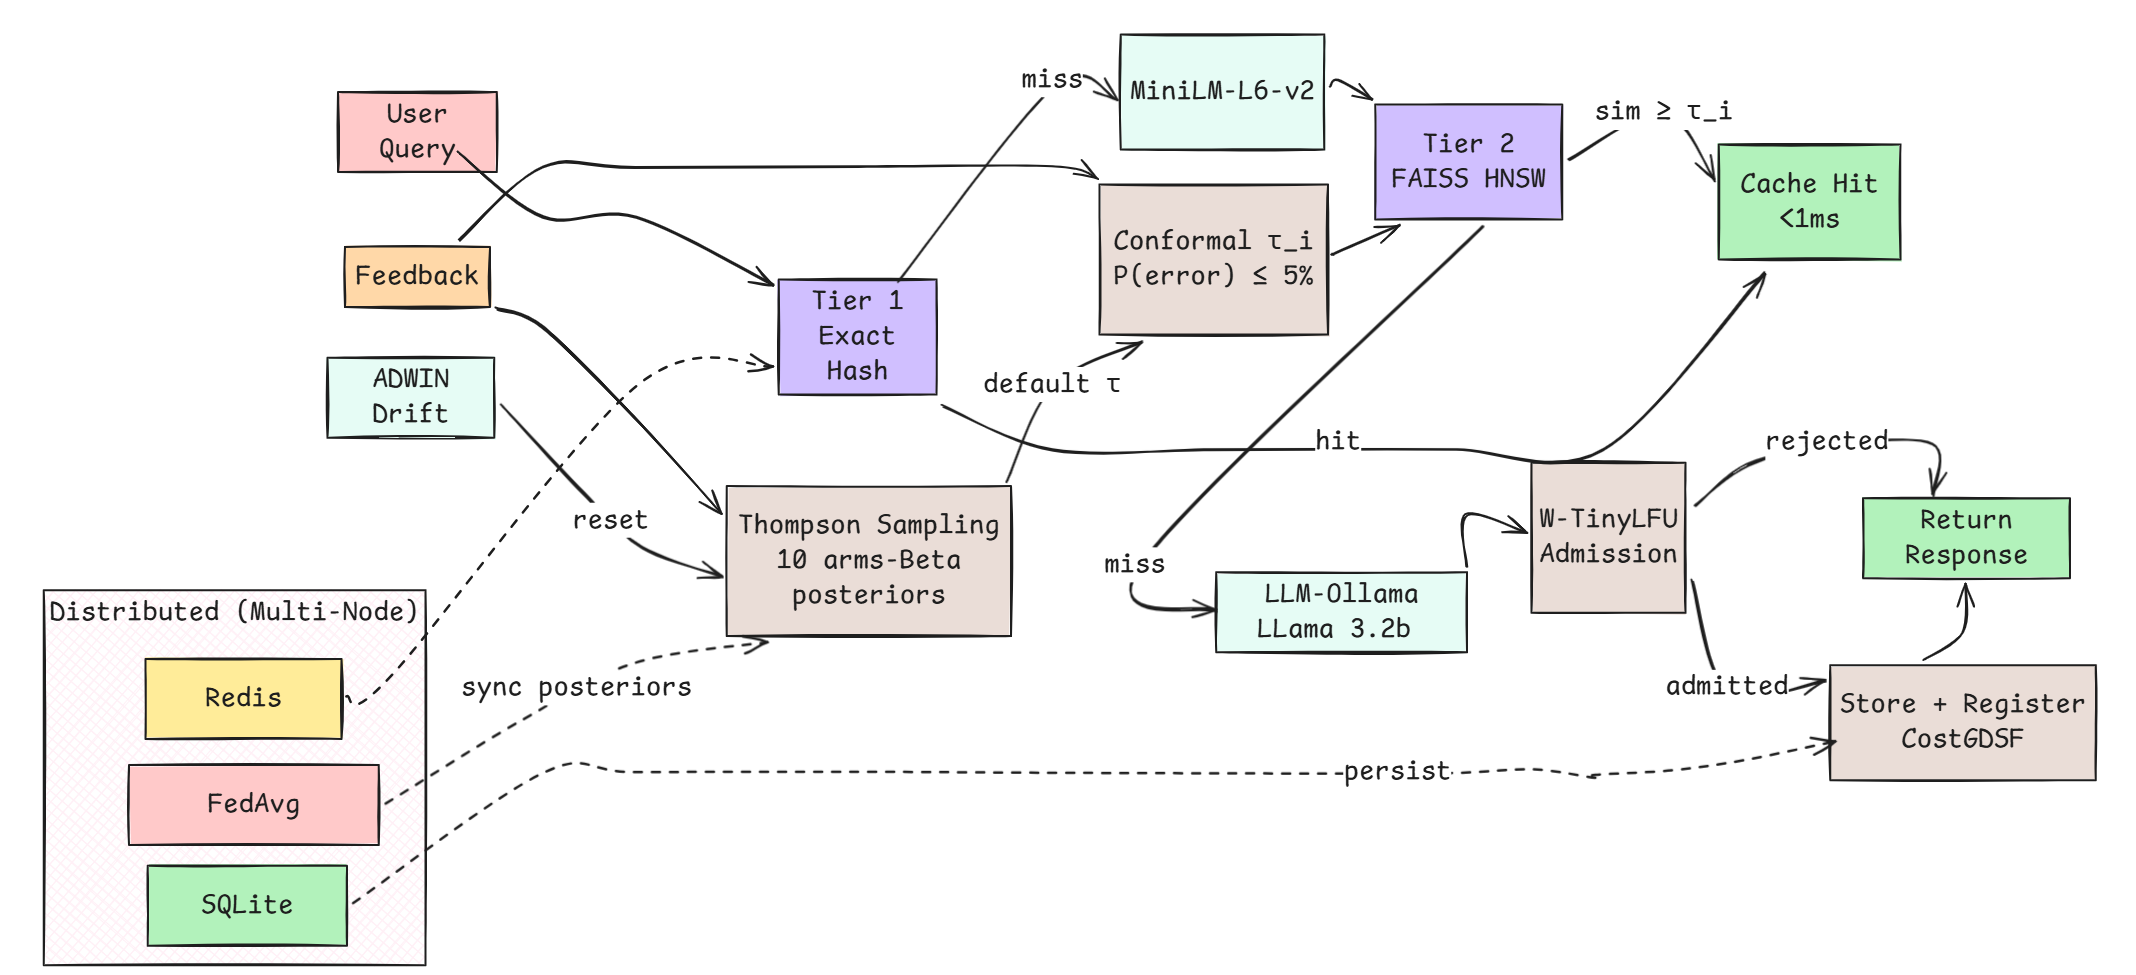
\includegraphics[width=\textwidth]{fig-architecture.png}
\caption{System Architecture Diagram}
\label{fig:architecture}
\end{figure}

Figure~\ref{fig:architecture} illustrates the complete data flow through the ContextualCache system. A user query enters from the top left and first passes through the Tier 1 exact hash lookup. On a miss, the query is encoded using the MiniLM-L6-v2 embedding model and forwarded to the Tier 2 FAISS HNSW index for semantic search. If a candidate exceeds its per-entry conformal threshold, the cached response is returned. Otherwise, the query falls through to the LLM backend, and the generated response passes through the W-TinyLFU admission gate before being stored with CostGDSF eviction metadata. The diagram also shows the feedback loop where correctness signals flow back to the conformal threshold calibrator, the Thompson Sampling bandit that learns optimal default thresholds, and the ADWIN drift detector that triggers bandit resets. On the left side, the distributed components are depicted: Redis for shared exact-match storage, FedAvg for bandit posterior synchronization, and SQLite for local persistence.

The central orchestrator is the ContextualCacheManager which coordinates all cache operations. When a query arrives, it flows through the following pipeline:

\begin{enumerate}[leftmargin=2cm]
\item \textbf{Tier 1 Exact Hash Lookup:} The query text is normalized (lowercased, punctuation stripped, whitespace collapsed) and hashed using SHA-256. The hash is checked against an in-memory dictionary and optionally against a Redis backing store. If found, the cached response is returned immediately with sub-millisecond latency.

\item \textbf{Embedding Generation:} If the exact hash lookup misses, the query is encoded into a 384-dimensional dense vector using the paraphrase-MiniLM-L6-v2 sentence transformer model. An LRU embedding cache (10,000 entries) avoids redundant encoding of recently seen queries.

\item \textbf{Session Context Fusion:} For multi-turn conversations, the query embedding is fused with the session context vector using exponential moving average with a query-dominant weight of $\alpha = 0.85$.

\item \textbf{Tier 2 Semantic Search:} The fused embedding is used to query a FAISS HNSW index that returns the top-$k$ (default $k=10$) nearest neighbors. For each candidate, the cosine similarity is computed and compared against the per-entry conformal threshold.

\item \textbf{Cache Hit or Miss Decision:} If any candidate exceeds its per-entry threshold, the cached response is returned. Otherwise, the query is forwarded to the LLM provider.

\item \textbf{LLM Fallback:} On cache miss, the query is sent to the configured LLM backend (Ollama, Groq, or OpenAI). The response is returned to the user and simultaneously processed for cache admission.

\item \textbf{Admission and Storage:} The new entry passes through the W-TinyLFU admission policy. If admitted, it is stored in both tiers with CostGDSF eviction metadata.
\end{enumerate}

\section{Query Pipeline Complexity}

\begin{table}[H]
\centering
\caption{Query Pipeline Complexity Analysis}
\label{tab:pipeline}
\begin{tabular}{llll}
\toprule
\textbf{Stage} & \textbf{Component} & \textbf{Complexity} & \textbf{Latency} \\
\midrule
Tier 1 & Exact Hash Lookup (SHA-256) & $O(1)$ & $<$1 ms \\
Tier 2 & FAISS HNSW Semantic Search & $O(\log n)$ & 2--15 ms \\
Embedding & paraphrase-MiniLM-L6-v2 & $O(d)$ & 5--20 ms \\
Threshold & Per-entry conformal $\tau_i$ & $O(k \log k)$ & $<$0.1 ms \\
Miss & LLM Provider (Ollama/Groq) & Network & 500--6000 ms \\
\bottomrule
\end{tabular}
\end{table}

\section{Cache Management Components}

\begin{table}[H]
\centering
\caption{Cache Management Component Summary}
\label{tab:components}
\begin{tabular}{p{3cm}p{4.5cm}p{6cm}}
\toprule
\textbf{Component} & \textbf{Algorithm} & \textbf{Purpose} \\
\midrule
Admission & Semantic W-TinyLFU & Reject one-hit-wonders based on LSH-bucketed frequency \\
Eviction & CostGDSF & $H = f \times c / s + L$ (keeps expensive entries) \\
Threshold Learning & Thompson Sampling (10 arms) & Learn optimal default $\tau$ for new entries \\
Drift Detection & ADWIN & Reset bandit posteriors on distribution shift \\
Session Context & EMA fusion ($\alpha$=0.85) & Multi-turn conversational awareness \\
Fault Isolation & Circuit Breaker & Per-dependency isolation (CLOSED/OPEN/HALF\_OPEN) \\
\bottomrule
\end{tabular}
\end{table}

\section{Two-Tier Lookup Architecture}

The two-tier lookup architecture is designed to minimize the average query latency. Tier 1 handles exact matches without requiring any embedding computation, saving approximately 5--20 milliseconds per query. Only on a Tier 1 miss does the system invoke the embedding model and FAISS index for Tier 2 semantic search.

The FAISS index uses the HNSW algorithm with the following parameters: $M=32$ links per node, $\text{efConstruction}=200$ for index build quality, and $\text{efSearch}=64$ for query-time accuracy. The index is wrapped in IndexIDMap2 for explicit ID management, allowing true vector removal. A periodic rebuild is triggered after every 500 removals to reclaim fragmented space.

\section{Per-Entry Conformal Thresholds}

The cornerstone of the proposed system is the per-entry conformal threshold mechanism. Unlike global-threshold approaches where a single value governs all cache hit decisions, our system maintains an individually calibrated threshold for each cached entry.

\textbf{Formulation:} For a cached entry with identifier $i$, the conformal threshold $\tau_i$ is computed as the $(1 - \varepsilon)$ quantile of the entry's nonconformity scores, where $\varepsilon$ is the target error rate (default 0.05). The nonconformity score for a query against entry $i$ is defined as:

For a correct cache hit with similarity $s$:
\begin{equation}
\text{nonconformity} = 1 - s
\end{equation}

For an incorrect cache hit with similarity $s$:
\begin{equation}
\text{nonconformity} = \min(1.0, \max(1 - s + 0.1, 0.5))
\end{equation}

\textbf{Calibration Process:} New entries start with a default threshold of 0.70. After accumulating at least 3 feedback signals, the threshold transitions to the conformal quantile computation. A sliding window of the most recent 200 nonconformity scores ensures adaptation to changing query patterns. The threshold is clamped to the range $[0.60, 0.99]$ to prevent extreme values.

\textbf{Formal Guarantee:} Under the exchangeability assumption of conformal prediction, the probability of a false positive satisfies:
\begin{equation}
P(\text{false positive}) \leq \varepsilon
\end{equation}

\textbf{Algorithm 1: Conformal Threshold Update}
\begin{lstlisting}
Input: entry_id, similarity, was_correct
If was_correct:
    nonconformity = 1.0 - similarity
Else:
    nonconformity = min(1.0, max(1.0 - similarity + 0.1, 0.5))

scores[entry_id].append(nonconformity)
If len(scores) > max_window:
    scores = scores[-max_window:]

If len(scores) >= min_calibration_points:
    sorted_scores = sort(scores)
    idx = ceil((1 - epsilon) * (len + 1)) - 1
    tau_i = 1.0 - sorted_scores[idx]
    tau_i = clamp(tau_i, 0.60, 0.99)
Else:
    tau_i = default_threshold
\end{lstlisting}

\section{Thompson Sampling Bandit for Threshold Exploration}

While conformal prediction provides per-entry fine-tuning after sufficient feedback, new entries initially use a default threshold. The Thompson Sampling bandit learns what this default should be by exploring different threshold values and observing their outcomes.

The bandit maintains 10 arms corresponding to threshold values linearly spaced from 0.65 to 0.95. Each arm $i$ has a Beta posterior $\alpha_i$ (successes) and $\beta_i$ (failures) params both init to 1.

\begin{table}[H]
\centering
\caption{Thompson Sampling Threshold Arms Configuration}
\label{tab:arms}
\begin{tabular}{cc}
\toprule
\textbf{Arm} & \textbf{Threshold Value} \\
\midrule
0 & 0.650 \\
1 & 0.683 \\
2 & 0.717 \\
3 & 0.750 \\
4 & 0.783 \\
5 & 0.817 \\
6 & 0.850 \\
7 & 0.883 \\
8 & 0.917 \\
9 & 0.950 \\
\bottomrule
\end{tabular}
\end{table}

\textbf{Algorithm 2: Thompson Sampling Update}
\begin{lstlisting}
On each cache hit:
    arm* = current best arm (highest expected reward)
    If similarity >= 0.85: reward = 1.0
    Else if similarity < 0.65: reward = 0.0
    Else: reward = (similarity - 0.65) / 0.20

    alpha[arm*] += reward
    beta[arm*] += (1.0 - reward)

    Feed reward to ADWIN drift detector
    If drift detected:
        Reset all alpha, beta to (2, 2)
\end{lstlisting}

The expected reward for each arm is computed as $\alpha_i / (\alpha_i + \beta_i)$, representing the empirical success rate. The arm with the highest expected reward determines the current best default threshold.

\section{ADWIN Drift Detection}

The ADWIN (Adaptive Windowing) algorithm monitors the stream of bandit rewards for distribution changes. It maintains a variable-length window of recent observations and uses Hoeffding bounds to test whether the means of two sub-windows differ significantly. When a drift is detected, the bandit posteriors are reset to weakly informative priors ($\alpha=2, \beta=2$), forcing renewed exploration.

\section{Semantic W-TinyLFU Admission Policy}

The admission policy determines whether a new entry should be admitted to the cache on a miss. The W-TinyLFU design consists of two stages:

\begin{enumerate}[leftmargin=2cm]
\item \textbf{Window Cache (5\% of capacity):} Admits all entries freely, providing a cold-start period where new entries can accumulate frequency without being rejected.
\item \textbf{Main Cache (95\% of capacity):} Requires that a new entry's frequency exceeds that of the window's LRU victim to gain admission.
\end{enumerate}

\textbf{Semantic Extension:} Rather than tracking frequency by exact query text, our system uses Random Projection LSH (8 bits, 4 tables) to map embedding vectors to discrete buckets. Semantically similar queries map to the same bucket, sharing a frequency counter in the Count-Min Sketch (width=4096, depth=4).

\section{CostGDSF Eviction}

When the cache reaches capacity and a new entry must be admitted, the CostGDSF policy selects the entry with the lowest priority score for eviction:

\begin{equation}
H(e) = \frac{\text{frequency}(e) \times \text{regen\_cost}(e)}{\text{storage\_bytes}(e)} + L
\end{equation}

where $\text{regen\_cost}(e) = (\text{llm\_cost\_usd} \times 10^6) + \text{embed\_cost\_ms}$ and $L$ is an inflation factor updated to the priority of the last evicted entry.

\section{Session Context Fusion}

For multi-turn conversations, the system maintains a session context accumulator. When a new query arrives within an active session, its embedding is fused with the accumulated context vector using exponential moving average:

\begin{equation}
\mathbf{c}_{\text{new}} = \alpha \cdot \mathbf{q} + (1 - \alpha) \cdot \mathbf{c}_{\text{old}}
\end{equation}

where $\alpha = 0.85$ (query-dominant). The fused vector is normalized to unit length before FAISS search. Sessions expire after 30 minutes of inactivity.

\section{Technology Stack}

\begin{table}[H]
\centering
\caption{Technology Stack}
\label{tab:techstack}
\begin{tabular}{ll}
\toprule
\textbf{Category} & \textbf{Technology} \\
\midrule
Language & Python 3.10 \\
Backend Framework & FastAPI with Uvicorn ASGI \\
Embedding Model & paraphrase-MiniLM-L6-v2 (384d) \\
Vector Index & FAISS (faiss-cpu) with HNSW \\
LLM Backend & Ollama (LLaMA 3.2:3b) / Groq / OpenAI \\
Optional Cache Store & Redis (redis-py async) \\
Persistence & SQLite \\
Frontend Framework & SvelteKit (Svelte 5) \\
Desktop Runtime & Tauri (Rust) \\
Charting & Chart.js \\
Deep Learning & PyTorch (CUDA 12.6) \\
Testing & pytest with pytest-asyncio (120 tests) \\
\bottomrule
\end{tabular}
\end{table}

\section{Backend Module Structure}

The backend is organized into the following Python modules within the \texttt{contextual\_cache} package:

\begin{itemize}[leftmargin=2cm]
\item \textbf{cache\_manager.py} --- Central orchestrator coordinating all cache operations, query pipeline, feedback processing, and statistics aggregation.
\item \textbf{lookup\_engine.py} --- Two-tier lookup with SHA-256 exact hash and FAISS IndexIDMap2(IndexHNSWFlat).
\item \textbf{embedding\_service.py} --- Sentence-transformers wrapper with LRU embedding cache.
\item \textbf{conformal\_thresholds.py} --- Per-entry conformal threshold store with online calibration.
\item \textbf{bandit.py} --- Thompson Sampling MAB with Beta posteriors and ADWIN integration.
\item \textbf{admission\_policy.py} --- Semantic W-TinyLFU with LSH-bucketed CMS frequency estimation.
\item \textbf{eviction.py} --- CostGDSF eviction with inflation factor tracking.
\item \textbf{drift\_detection.py} --- ADWIN drift detector using Hoeffding bounds.
\item \textbf{circuit\_breaker.py} --- Per-dependency circuit breaker (CLOSED/OPEN/HALF\_OPEN).
\item \textbf{session\_context.py} --- Session context accumulator with EMA fusion.
\item \textbf{llm\_provider.py} --- Unified LLM abstraction over Ollama, Groq, and OpenAI.
\item \textbf{redis\_store.py} --- Optional Redis-backed exact-match store with circuit breaker.
\item \textbf{persistence.py} --- SQLite persistence for cache entries, scores, bandit state, and chat history.
\item \textbf{metrics.py} --- Metrics collector powering the dashboard.
\item \textbf{data\_structures.py} --- CMS, LSH, LRU, and SLRU implementations.
\item \textbf{config.py} --- Pydantic BaseSettings with CC\_ environment variable overrides.
\end{itemize}

\section{API Endpoints}

\begin{table}[H]
\centering
\caption{API Endpoint Summary}
\label{tab:api}
\begin{tabular}{lll}
\toprule
\textbf{Method} & \textbf{Path} & \textbf{Description} \\
\midrule
POST & /query & Main cache-fronted LLM query \\
POST & /feedback & Correctness feedback for calibration \\
POST & /bulk-query & Batch queries \\
POST & /api/query-direct & Bypass cache, call LLM directly \\
GET & /health & Health check \\
GET & /api/stats & Full analytics for dashboard \\
POST & /api/clear-cache & Clear all cache entries \\
GET & /api/conversations & List chat sessions \\
POST & /api/benchmark/run & Start benchmark run \\
GET & /api/benchmark/status/\{id\} & Poll benchmark progress \\
GET & /api/benchmark/results & List benchmark results \\
\bottomrule
\end{tabular}
\end{table}

\section{Frontend Dashboard}

The frontend is built as a cross-platform desktop application using Tauri (Rust runtime) with SvelteKit (Svelte 5) and Chart.js for visualization. It features a dark-themed interface with four main pages:

\textbf{Chat Interface:} A conversational interface with session management, cache hit/miss metadata display, token usage tracking, and a collapsible conversation history sidebar. Sessions are persisted via the backend SQLite database.

\textbf{Cache Comparison View:} A side-by-side comparison tool that simultaneously queries the cache and the LLM directly, displaying latency, token count, and speedup metrics.

\textbf{Analytics Dashboard:} A real-time analytics page displaying six key performance indicators, hit rate trends, query tier breakdown, latency time series, Thompson Sampling arm distribution, and similarity distribution. The dashboard polls the backend every three seconds.

\textbf{Benchmark Suite:} An integrated benchmark runner with configurable parameters (number of questions, cache capacity, dataset selection between NQ and SQuAD), real-time progress tracking, and results visualization.

Screenshots of all four pages are presented in Section 4.7.

\section{Benchmark Framework}

The benchmark system compares ContextualCache against six baseline strategies under identical conditions:

\begin{enumerate}[leftmargin=2cm]
\item \textbf{Exact-Match LRU} --- Hash-based exact matching with LRU eviction (lower-bound baseline).
\item \textbf{GPTCache} --- Static threshold (0.75) with LRU eviction [3].
\item \textbf{MeanCache} --- Adaptive threshold (mean $-$ std) with PCA compression and LRU [2].
\item \textbf{vCache} --- Per-entry conformal thresholds with LRU eviction [4].
\item \textbf{RAGCache} --- Static threshold (0.85) with cost-aware GDSF eviction [8].
\item \textbf{No-Admission} --- Conformal thresholds with CostGDSF but no admission gate (ablation study).
\end{enumerate}

All strategies receive identical pre-computed embeddings and LLM responses to ensure fair comparison.

\section{Testing}

The system includes 120 automated tests organized across 12 test files, all executed through pytest with the pytest-asyncio plugin running in auto mode so that asynchronous test functions are handled transparently. The test suite was designed to cover every major component of the system in isolation, ensuring that individual modules behave correctly before they are wired together in the cache manager.

The data structures tests in \texttt{test\_data\_structures.py} verify the Count-Min Sketch implementation including conservative updates, frequency halving for aging, and the property that estimates never undercount. The same file tests the Random Projection LSH hash function for determinism and collision properties, and validates both the LRU and Segmented LRU eviction data structures for correct ordering and capacity enforcement.

The session context tests verify that the EMA fusion formula produces the expected blended vectors when given known inputs, that session expiration occurs after the configured inactivity timeout, and that creating a new session produces a fresh context vector uncontaminated by prior sessions.

Conformal threshold tests check the core calibration logic: that the threshold converges toward the correct quantile as feedback accumulates, that the clamping bounds of 0.60 and 0.99 are respected even when the raw quantile falls outside that range, and that entries with fewer than the minimum calibration points fall back to the default threshold rather than producing unstable estimates.

The eviction and admission tests exercise CostGDSF priority computation with known frequency, cost, and size values to verify the priority formula, and test that W-TinyLFU correctly rejects low-frequency candidates while admitting high-frequency ones. The fault tolerance tests cover the circuit breaker state machine transitions between CLOSED, OPEN, and HALF\_OPEN states, ADWIN drift detection with synthetic distribution shifts, and Thompson Sampling arm selection with controlled reward sequences.

The lookup engine tests are among the most critical, verifying that stored entries can be retrieved by both exact hash and semantic search, that FAISS ID mapping is consistent after insertions and deletions, that the periodic index rebuild produces correct results, and that text normalization is applied consistently so that ``What is AI?'' and ``what is ai'' map to the same hash. TTL expiration is also tested by inserting entries with short time-to-live values and confirming they are excluded from search results after expiration.

Persistence tests round-trip cache entries through the SQLite layer, checking that embeddings survive serialization with full floating-point fidelity, that bandit posteriors and conformal scores are correctly saved and restored, and that conversation history can be created, queried, and deleted without data corruption.

The remaining test files cover configuration validation (rejecting invalid capacity or threshold values), rate limiter token bucket behavior and per-tenant isolation, consistent hash ring distribution and node addition/removal stability, vector clock ordering and merge semantics, and write-ahead log append/replay with CRC integrity verification and checkpoint-based LSN recovery.

All tests run without network access or GPU requirements, using lightweight in-memory instances of each component. The full suite completes in under 15 seconds on a standard development machine.

\section{Distributed Systems Design}

Although the primary evaluation in this report focuses on a single-node deployment, the system includes a complete set of distributed systems components designed for future multi-node scaling. These components were developed and unit-tested alongside the core cache logic to ensure architectural readiness for horizontal scaling.

The consistent hashing module implements a SHA-256-based hash ring with configurable virtual nodes (default 150 per physical node). Virtual nodes spread each physical node's responsibility across many points on the ring, reducing the variance in load distribution. When a node is added or removed, only the keys that fall in the affected arc of the ring need to be reassigned, minimizing data movement. The implementation supports dynamic node addition and removal, and the unit tests verify that key ownership changes are bounded and predictable.

The write-ahead log provides crash recovery guarantees for cache mutations. Every store, remove, and threshold update operation is first appended to a sequential log file with a CRC32 integrity checksum before it is applied to the in-memory cache. On startup, the system replays any log entries written after the last checkpoint to reconstruct the cache state. Periodic checkpoints truncate the log to prevent unbounded growth. The WAL uses monotonically increasing log sequence numbers so that replay is idempotent even if the process crashed mid-write.

Vector clocks provide causal ordering for distributed cache operations. Each node maintains a logical timestamp vector, and every cache mutation is tagged with the current vector clock. When two nodes exchange state, they can determine whether one update causally precedes another or whether the updates are concurrent and require conflict resolution. The implementation supports increment, merge, and happens-before comparison operations.

The gossip protocol enables decentralized synchronization of Thompson Sampling bandit posteriors across cache nodes. Each node periodically selects a random peer and exchanges its current bandit state using a push-pull protocol. The received posteriors are merged using Federated Averaging, where the alpha and beta parameters from both nodes are averaged to produce a combined posterior that reflects the collective experience of the cluster. This approach avoids the need for a central coordinator and is tolerant of node failures and network partitions.

\section{Configuration Parameters}

\begin{table}[H]
\centering
\caption{Configuration Parameters}
\label{tab:config}
\begin{tabular}{lll}
\toprule
\textbf{Parameter} & \textbf{Value} & \textbf{Description} \\
\midrule
CC\_CACHE\_CAPACITY & 50,000 & Max cached entries (300 for benchmark) \\
CC\_DEFAULT\_THRESHOLD & 0.70 & Initial conformal threshold \\
CC\_TARGET\_ERROR\_RATE & 0.05 & Conformal error bound ($\varepsilon$) \\
CC\_EMBEDDING\_MODEL & MiniLM-L6-v2 & 384-dimensional embeddings \\
CC\_ANN\_K & 10 & FAISS top-$k$ neighbors \\
CC\_HNSW\_M & 32 & HNSW links per node \\
CC\_HNSW\_EF\_SEARCH & 64 & HNSW search expansion \\
CC\_WINDOW\_PCT & 0.05 & W-TinyLFU window fraction \\
CC\_CMS\_WIDTH & 4096 & Count-Min Sketch columns \\
CC\_BANDIT\_N\_ARMS & 10 & Thompson Sampling arms \\
CC\_DRIFT\_DELTA & 0.002 & ADWIN sensitivity \\
CC\_DEFAULT\_TTL\_S & 3600 & Entry time-to-live (seconds) \\
\bottomrule
\end{tabular}
\end{table}


% ════════════════════════════════════════════════════════════
% CHAPTER 4: RESULTS AND DISCUSSION
% ════════════════════════════════════════════════════════════
\chapter{Results and Discussion}

\section{Experimental Setup}

\textbf{Datasets:} Two public question-answering datasets from HuggingFace were used for evaluation:

\begin{enumerate}[leftmargin=2cm]
\item \textbf{Natural Questions (NQ)} --- Google's Natural Questions dataset containing web search queries with short answers. 500 unique questions were sampled with 150 paraphrase variants (30\% ratio) for a total of 650 queries per run.
\item \textbf{SQuAD} --- Stanford Question Answering Dataset (validation split) containing reading comprehension questions. 500 unique questions with 150 paraphrases, totaling 650 queries.
\end{enumerate}

\textbf{Paraphrase Generation:} Deterministic rule-based transforms were applied to generate paraphrase variants. The system implements 26 transformation patterns including syntactic restructuring and prefix injection.

\textbf{Configuration:} Cache capacity was set to 300 entries. The LLM backend was Ollama running LLaMA 3.2:3b locally. All embeddings were pre-computed and shared across all strategies.

\textbf{Metrics:}
\begin{itemize}[leftmargin=2cm]
\item \textbf{Hit Rate} = total\_hits / total\_queries
\item \textbf{Precision} = correct\_hits / total\_hits
\item \textbf{F1 Score} = $2 \times \text{precision} \times \text{recall} / (\text{precision} + \text{recall})$
\item \textbf{LLM Calls} = number of queries forwarded to the LLM
\end{itemize}

\section{Results on Natural Questions}

\begin{table}[H]
\centering
\caption{Benchmark Results on Natural Questions Dataset (650 queries, 300 capacity)}
\label{tab:nq}
\begin{tabular}{lcccccc}
\toprule
\textbf{Strategy} & \textbf{Hit Rate} & \textbf{Precision} & \textbf{F1} & \textbf{Correct} & \textbf{Incorrect} & \textbf{LLM Calls} \\
\midrule
\textbf{Ours} & \textbf{20.77\%} & \textbf{62.22\%} & \textbf{0.214} & \textbf{84} & \textbf{51} & \textbf{515} \\
GPTCache & 19.38\% & 61.90\% & 0.201 & 78 & 48 & 524 \\
vCache & 18.62\% & 62.81\% & 0.197 & 76 & 45 & 529 \\
No-Admission & 17.69\% & 63.48\% & 0.191 & 73 & 42 & 535 \\
RAGCache & 17.23\% & 64.29\% & 0.189 & 72 & 40 & 538 \\
MeanCache & 13.23\% & 66.28\% & 0.155 & 57 & 29 & 564 \\
Exact-Match LRU & 0.00\% & --- & 0.000 & 0 & 0 & 650 \\
\bottomrule
\end{tabular}
\end{table}

\begin{figure}[H]
\centering
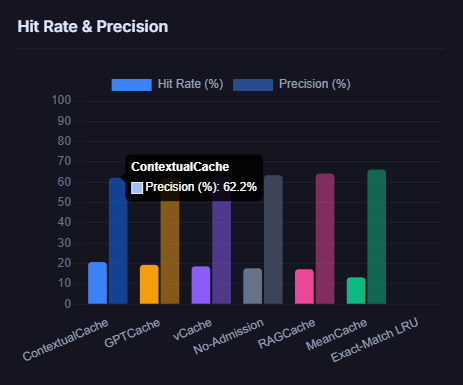
\includegraphics[width=0.85\textwidth]{fig-hit-rate-precision-chart.png}
\caption{Hit Rate and Precision Comparison across Strategies (NQ Dataset)}
\label{fig:hitrate}
\end{figure}

Figure~\ref{fig:hitrate} presents a grouped bar chart comparing the hit rate and precision of all seven strategies on the Natural Questions dataset. Each strategy has two bars: a blue bar for hit rate and a purple bar for precision. ContextualCache leads with a 20.77\% hit rate paired with 62.2\% precision, followed by GPTCache at 19.38\% and vCache at 18.62\%. MeanCache shows the lowest semantic hit rate at 13.23\% but achieves the highest precision at 66.28\%, reflecting its conservative threshold. Exact-Match LRU records zero hits, confirming that no benchmark queries are textually identical to cached entries.

The results demonstrate that ContextualCache achieves the highest hit rate (20.77\%) and the highest F1 score (0.214) among all strategies. Compared to GPTCache, ContextualCache serves 6 additional correct cache hits (84 vs 78) while saving 9 more LLM calls (515 vs 524). The precision of 62.22\% is competitive with GPTCache's 61.90\%, indicating that the higher hit rate does not come at the cost of increased false positives.

The lower default threshold (0.70) allows ContextualCache to capture paraphrase matches that GPTCache (threshold 0.75) and RAGCache (threshold 0.85) miss. The per-entry conformal calibration then tightens individual thresholds based on feedback, preventing the lower default from degrading precision.

MeanCache achieves the highest precision (66.28\%) but at the cost of a significantly lower hit rate (13.23\%), as its adaptive threshold (mean $-$ std) tends to be conservative.

\section{Results on SQuAD}

\begin{table}[H]
\centering
\caption{Benchmark Results on SQuAD Dataset (650 queries, 300 capacity)}
\label{tab:squad}
\begin{tabular}{lcccccc}
\toprule
\textbf{Strategy} & \textbf{Hit Rate} & \textbf{Precision} & \textbf{F1} & \textbf{Correct} & \textbf{Incorrect} & \textbf{LLM Calls} \\
\midrule
\textbf{Ours} & \textbf{23.69\%} & 35.71\% & \textbf{0.137} & \textbf{55} & 99 & \textbf{496} \\
GPTCache & 19.54\% & 38.58\% & 0.126 & 49 & 78 & 523 \\
vCache & 17.85\% & 38.79\% & 0.118 & 45 & 71 & 534 \\
No-Admission & 17.85\% & 37.07\% & 0.112 & 43 & 73 & 534 \\
RAGCache & 17.38\% & 36.28\% & 0.108 & 41 & 72 & 537 \\
MeanCache & 5.23\% & 47.06\% & 0.047 & 16 & 18 & 616 \\
Exact-Match LRU & 0.00\% & --- & 0.000 & 0 & 0 & 650 \\
\bottomrule
\end{tabular}
\end{table}

On SQuAD, ContextualCache again achieves the highest hit rate (23.69\%) and F1 score (0.137), outperforming GPTCache by 4.15 percentage points in hit rate. The overall precision is lower across all strategies on SQuAD compared to NQ, reflecting the challenge of matching short, factual SQuAD answers within longer LLM-generated responses. ContextualCache saves 154 LLM calls out of 650 queries on SQuAD, the most among all strategies.

\section{Precision Analysis}

\begin{table}[H]
\centering
\caption{Precision Analysis on NQ --- Top Three Strategies}
\label{tab:precision}
\begin{tabular}{lccc}
\toprule
\textbf{Metric} & \textbf{GPTCache} & \textbf{vCache} & \textbf{Ours} \\
\midrule
Total Hits & 126 & 121 & 135 \\
Correct Hits & 78 & 76 & 84 \\
Incorrect Hits & 48 & 45 & 51 \\
Precision & 61.90\% & 62.81\% & 62.22\% \\
False Positive Rate & 38.10\% & 37.19\% & 37.78\% \\
\bottomrule
\end{tabular}
\end{table}

ContextualCache serves 84 correct responses out of 135 total hits, meaning that approximately 62\% of cache hits deliver the right answer. GPTCache achieves a similar precision (61.90\%) but with fewer total hits (126). The marginal difference in precision (0.32 percentage points) is offset by the significant advantage in hit rate (1.39 percentage points) and total correct hits (6 more).

\section{Latency Analysis}

\begin{table}[H]
\centering
\caption{Latency Comparison on NQ}
\label{tab:latency}
\begin{tabular}{lccc}
\toprule
\textbf{Strategy} & \textbf{Hit Latency (ms)} & \textbf{Overall Latency (ms)} & \textbf{LLM Saved} \\
\midrule
Ours & 0.00 & 1610.17 & 135 \\
GPTCache & 0.13 & 1613.17 & 126 \\
vCache & 0.00 & 1632.40 & 121 \\
No-Admission & 0.13 & 1662.86 & 115 \\
RAGCache & 0.28 & 1675.60 & 112 \\
MeanCache & 0.00 & 1736.22 & 86 \\
\bottomrule
\end{tabular}
\end{table}

\begin{figure}[H]
\centering
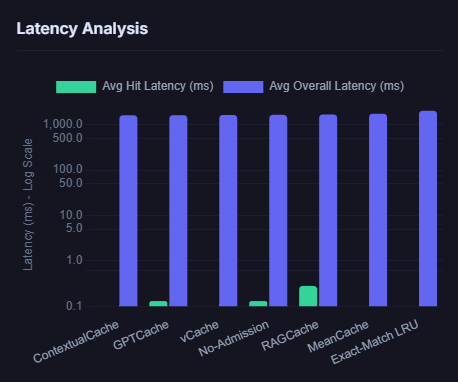
\includegraphics[width=0.85\textwidth]{fig-latency-chart.png}
\caption{Latency Analysis across Strategies (Log Scale)}
\label{fig:latency}
\end{figure}

Figure~\ref{fig:latency} uses a logarithmic y-axis to display two latency metrics for each strategy: average hit latency (green bars) and average overall latency (purple bars). The log scale is necessary because hit latencies are sub-millisecond while overall latencies exceed 1000 milliseconds. All strategies show similar overall latencies around 1600--2000 milliseconds, since this metric is dominated by LLM inference time on cache misses. The green hit latency bars are visible only for GPTCache, No-Admission, and RAGCache at fractions of a millisecond, while the remaining strategies report effectively zero hit latency.

All strategies achieve sub-millisecond hit latency, confirming that cache lookup overhead is negligible compared to LLM inference. ContextualCache achieves the lowest overall latency (1610.17 ms) due to its highest hit rate.

\section{Thompson Sampling Arm Distribution}

The Thompson Sampling bandit provides insights into the optimal threshold region. After processing cache queries, the arm distribution shows the learned expected rewards for each threshold value, with lower thresholds generally receiving higher rewards due to their ability to capture more valid semantic matches.

\section{Cross-Dataset Comparison}

Comparing the results across the two datasets reveals important patterns about how the cache behaves under different workload characteristics. On Natural Questions, which contains diverse web search queries spanning many topics, the system achieves 20.77\% hit rate with 62.22\% precision. On SQuAD, which contains reading comprehension questions that are more narrowly focused on specific Wikipedia passages, the hit rate rises to 23.69\% but precision drops to 35.71\%.

The higher hit rate on SQuAD can be attributed to the nature of the questions themselves. SQuAD questions are derived from a fixed set of passages, so multiple questions about the same passage tend to share vocabulary and structure, producing higher embedding similarity scores. This means the cache encounters more queries that fall within the similarity radius of existing entries. However, the lower precision reveals the other side of this coin: SQuAD questions about the same passage often ask about different specific facts, so a high similarity score does not reliably indicate that the cached answer is correct for the new question. Two questions like ``Who founded the university?'' and ``When was the university founded?'' may have very similar embeddings but require entirely different answers.

On Natural Questions, the queries are more topically diverse since they come from real web searches rather than a fixed document collection. This diversity means fewer queries fall close enough to existing entries to trigger a cache hit, explaining the lower hit rate. But when a hit does occur, the broader topical spread means the matching query is more likely to be a genuine paraphrase rather than a superficially similar but semantically distinct question, which is why precision is substantially higher.

This cross-dataset analysis highlights an important practical consideration for deploying the cache: the relationship between hit rate and precision depends heavily on the characteristics of the incoming query stream. Applications with repetitive, narrow question patterns will see higher hit rates but may need stricter thresholds to maintain acceptable precision. Applications with diverse, broad queries will naturally achieve lower hit rates but can afford more relaxed thresholds because the hits that do occur tend to be genuine matches.

\section{Ablation Analysis}

The No-Admission baseline serves as a direct ablation of the W-TinyLFU admission policy. It uses the same conformal thresholds and CostGDSF eviction as the full ContextualCache system but admits every entry unconditionally on a cache miss. Comparing ContextualCache (20.77\% hit rate, 62.22\% precision on NQ) against No-Admission (17.69\% hit rate, 63.48\% precision) isolates the contribution of the admission policy.

The admission gate improves hit rate by 3.08 percentage points while reducing precision by only 1.26 percentage points. This improvement arises because the frequency-gated admission prevents one-time queries from consuming cache capacity that could be used by entries with higher reuse potential. By keeping the cache populated with entries that have demonstrated at least some frequency signal, the system increases the probability that future queries will find a relevant match.

The slight precision decrease is expected: the admission policy allows more entries into the cache overall, which broadens the set of potential matches and increases the chance of a near-miss being incorrectly served. However, the net effect on F1 score is clearly positive (0.214 versus 0.191), indicating that the additional correct hits outweigh the marginal increase in false positives.

The comparison between vCache and ContextualCache further isolates the combined effect of the Thompson Sampling bandit, CostGDSF eviction, and admission policy. vCache uses the same conformal threshold mechanism but with a higher default threshold of 0.80, simple LRU eviction, and no admission control. ContextualCache outperforms vCache by 2.15 percentage points in hit rate on NQ, demonstrating that the bandit's learned lower default threshold (around 0.70) captures valid matches that vCache's conservative default misses.

\section{Cost Savings Estimation}

To put the benchmark results into a practical context, consider the cost implications of deploying this cache in a production environment. On the NQ workload, ContextualCache saves 135 LLM inference calls out of 650 queries, a savings rate of 20.77\%. If we project this to a service handling 100,000 queries per day using a cloud LLM provider, the cache would eliminate approximately 20,770 LLM calls daily.

Using OpenAI's GPT-4 pricing as a reference point (approximately 0.03 USD per 1,000 input tokens and 0.06 USD per 1,000 output tokens), and assuming an average of 50 input tokens and 200 output tokens per query, each saved LLM call avoids roughly 0.0135 USD in inference cost. At 20,770 saved calls per day, the daily cost savings would amount to approximately 280 USD, translating to over 8,400 USD per month. Even with more affordable models like GPT-3.5-turbo, the savings remain meaningful at scale.

Beyond direct monetary savings, there is a latency benefit. Each cache hit avoids a round trip to the LLM provider that would take between 500 milliseconds and 6 seconds. At a 20.77\% hit rate, roughly one in five user requests receives a response in under 1 millisecond instead of waiting for the LLM. For interactive applications where perceived responsiveness drives user engagement, this improvement in tail latency has a tangible impact on user experience that goes beyond what the raw cost numbers capture.

\section{False Positive Analysis}

A false positive occurs when the cache serves a response for a query that is semantically similar to the cached entry but requires a different answer. Across all strategies on NQ, false positive rates range from 33.72\% (MeanCache) to 38.10\% (GPTCache). ContextualCache sits at 37.78\%, which is slightly better than GPTCache despite having a more aggressive threshold.

It is important to note that the false positive rate in this benchmark is inflated by the evaluation methodology. The benchmark treats any cache hit where the cached response does not contain the exact gold answer string as incorrect, even if the cached response is a reasonable and factually accurate answer to the query. For instance, if the gold answer is ``Paris'' and the cached response says ``The capital of France is Paris, which is located in the north-central part of the country,'' a simple string containment check would correctly identify this as a true positive. But if the gold answer is a specific date format like ``January 15, 1929'' and the cached response uses a different format or provides additional context, the evaluation may flag it as incorrect despite the response being substantively accurate.

In a production deployment with actual users, the effective false positive rate would likely be lower because users have broader acceptance criteria than exact string matching. The conformal threshold mechanism is specifically designed to reduce false positives over time as feedback accumulates, so the single-pass benchmark numbers represent a worst case before the system has had the opportunity to calibrate individual entry thresholds through repeated use.

\section{Implementation Demonstration}

The implemented system was tested through interactive usage to validate end-to-end functionality. The following screenshots demonstrate the four main dashboard pages.

\begin{figure}[H]
\centering
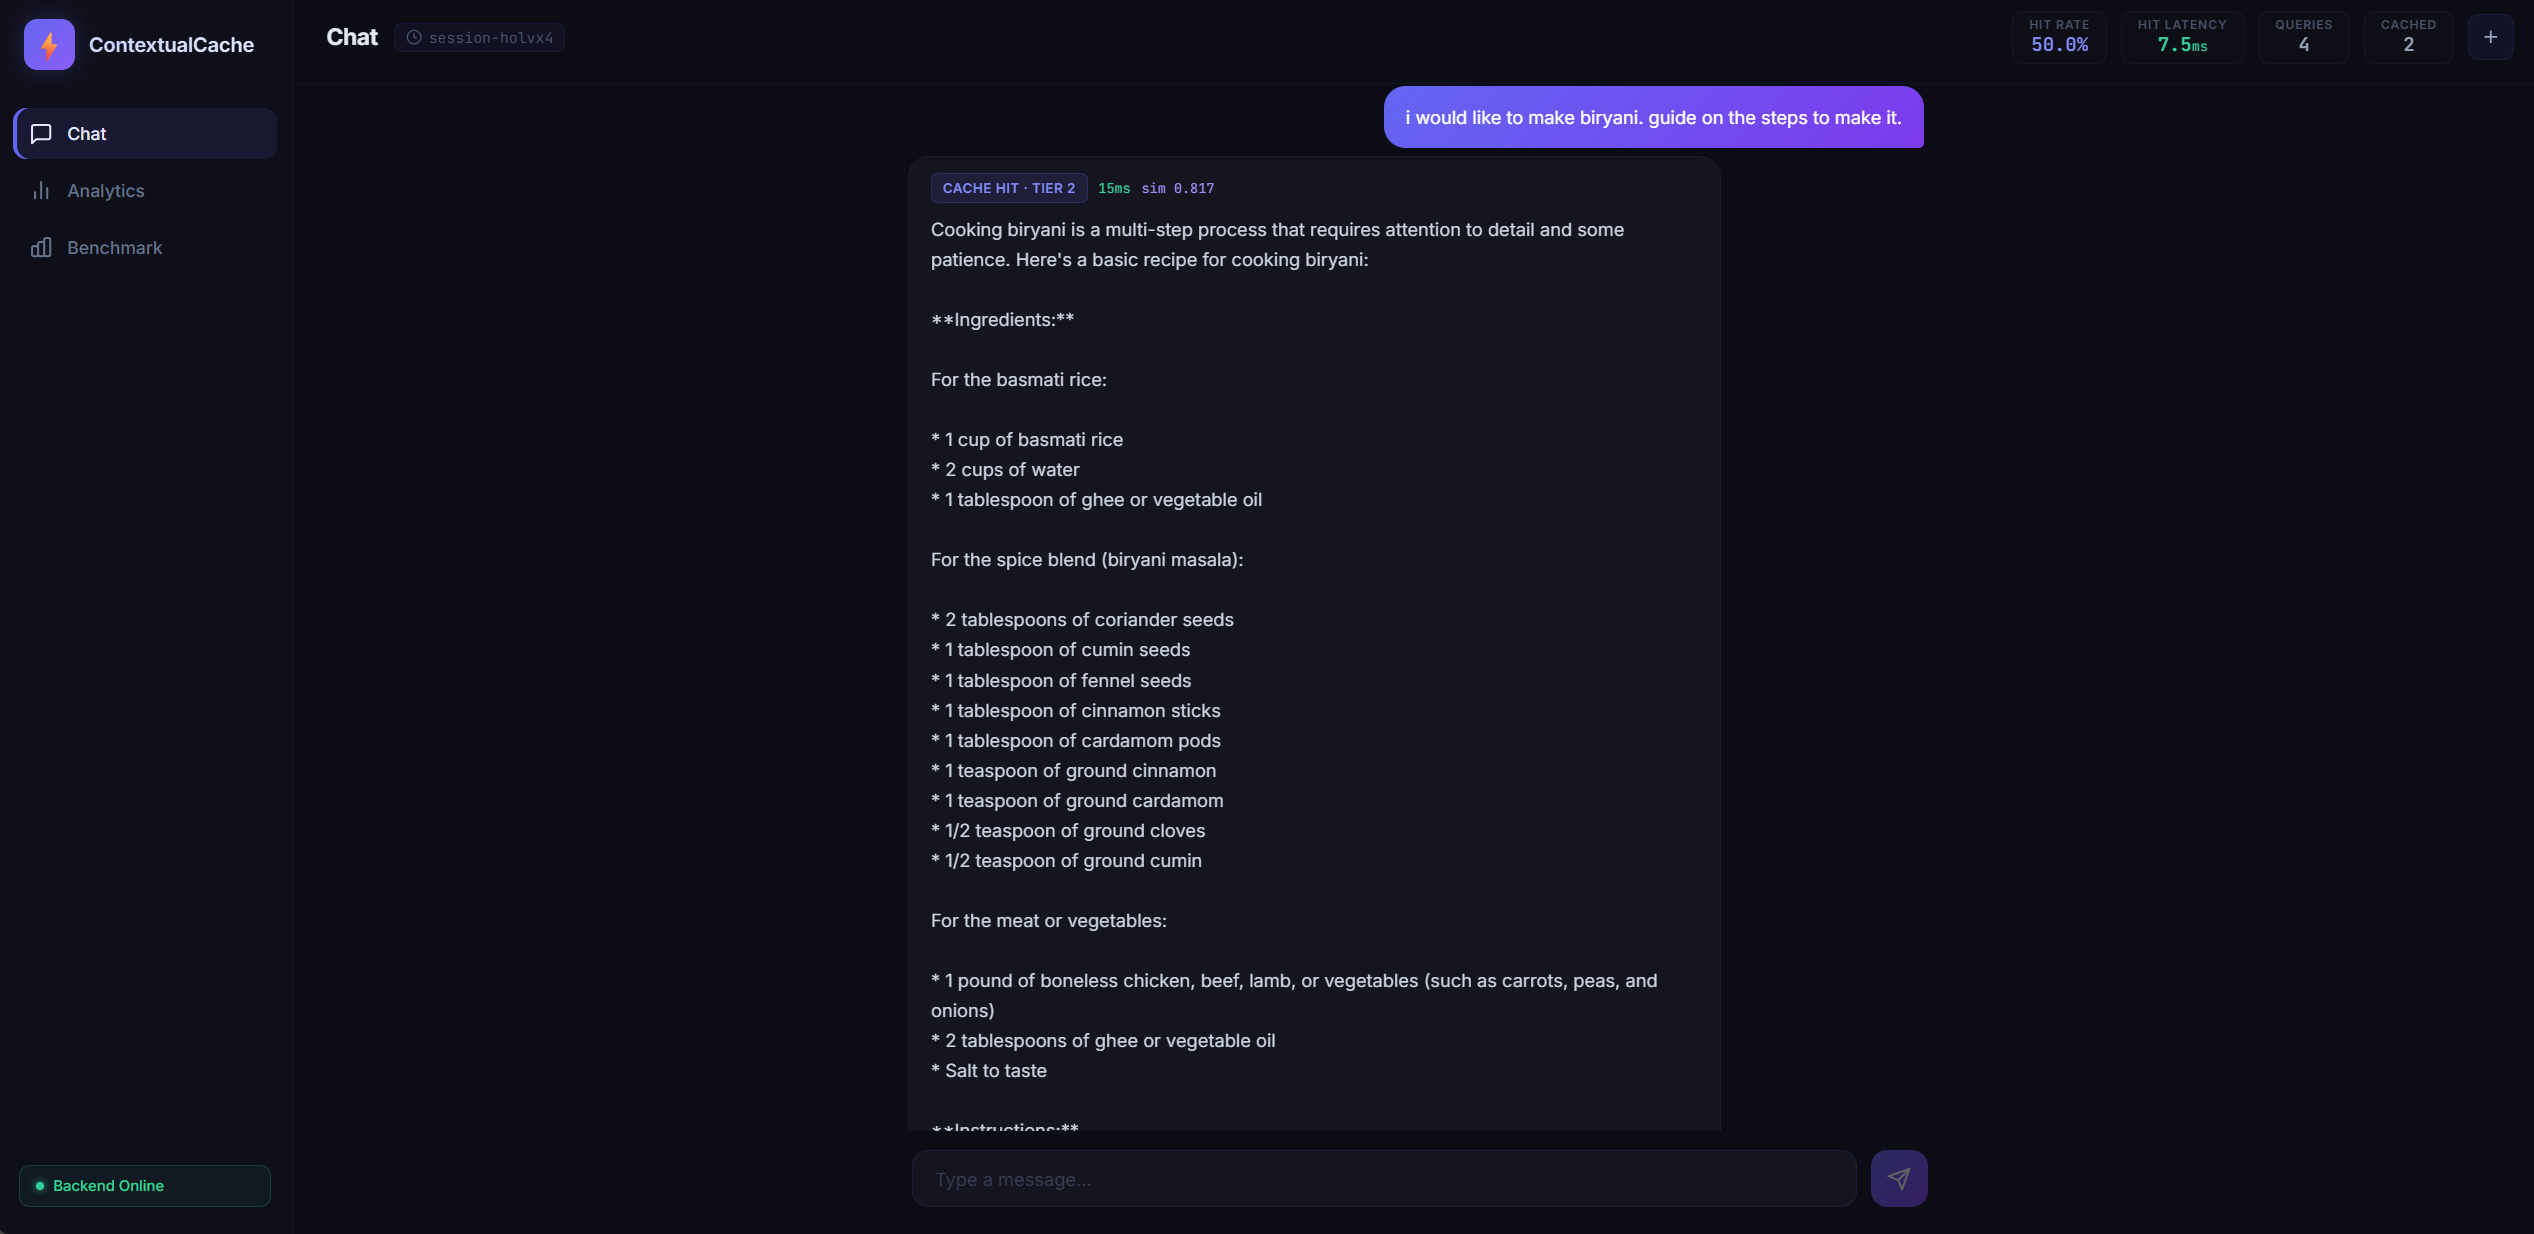
\includegraphics[width=1.0\textwidth]{fig-chat-interface.png}
\caption{Chat Interface demonstrating cache hit/miss behavior}
\label{fig:chat}
\end{figure}

Figure~\ref{fig:chat} shows the main chat interface of the ContextualCache dashboard. The left sidebar provides navigation across the four pages --- Chat, Analytics, and Benchmark --- along with a backend connectivity indicator at the bottom. At the top of the screen, key performance indicators are displayed in real time, including the current hit rate of 50.0\%, hit latency of 7.5 milliseconds, total queries processed, and the number of cached entries. In this demonstration, the user has asked for a biryani recipe. The response is tagged with a green ``Cache Hit -- Tier 2'' label, indicating that it was served from the FAISS semantic search tier rather than being generated fresh by the LLM. The metadata alongside the tag shows a similarity score of 0.817 and a response time of 15 milliseconds, confirming that the system successfully matched the query to a semantically similar cached entry and returned the result with minimal latency.

\begin{figure}[H]
\centering
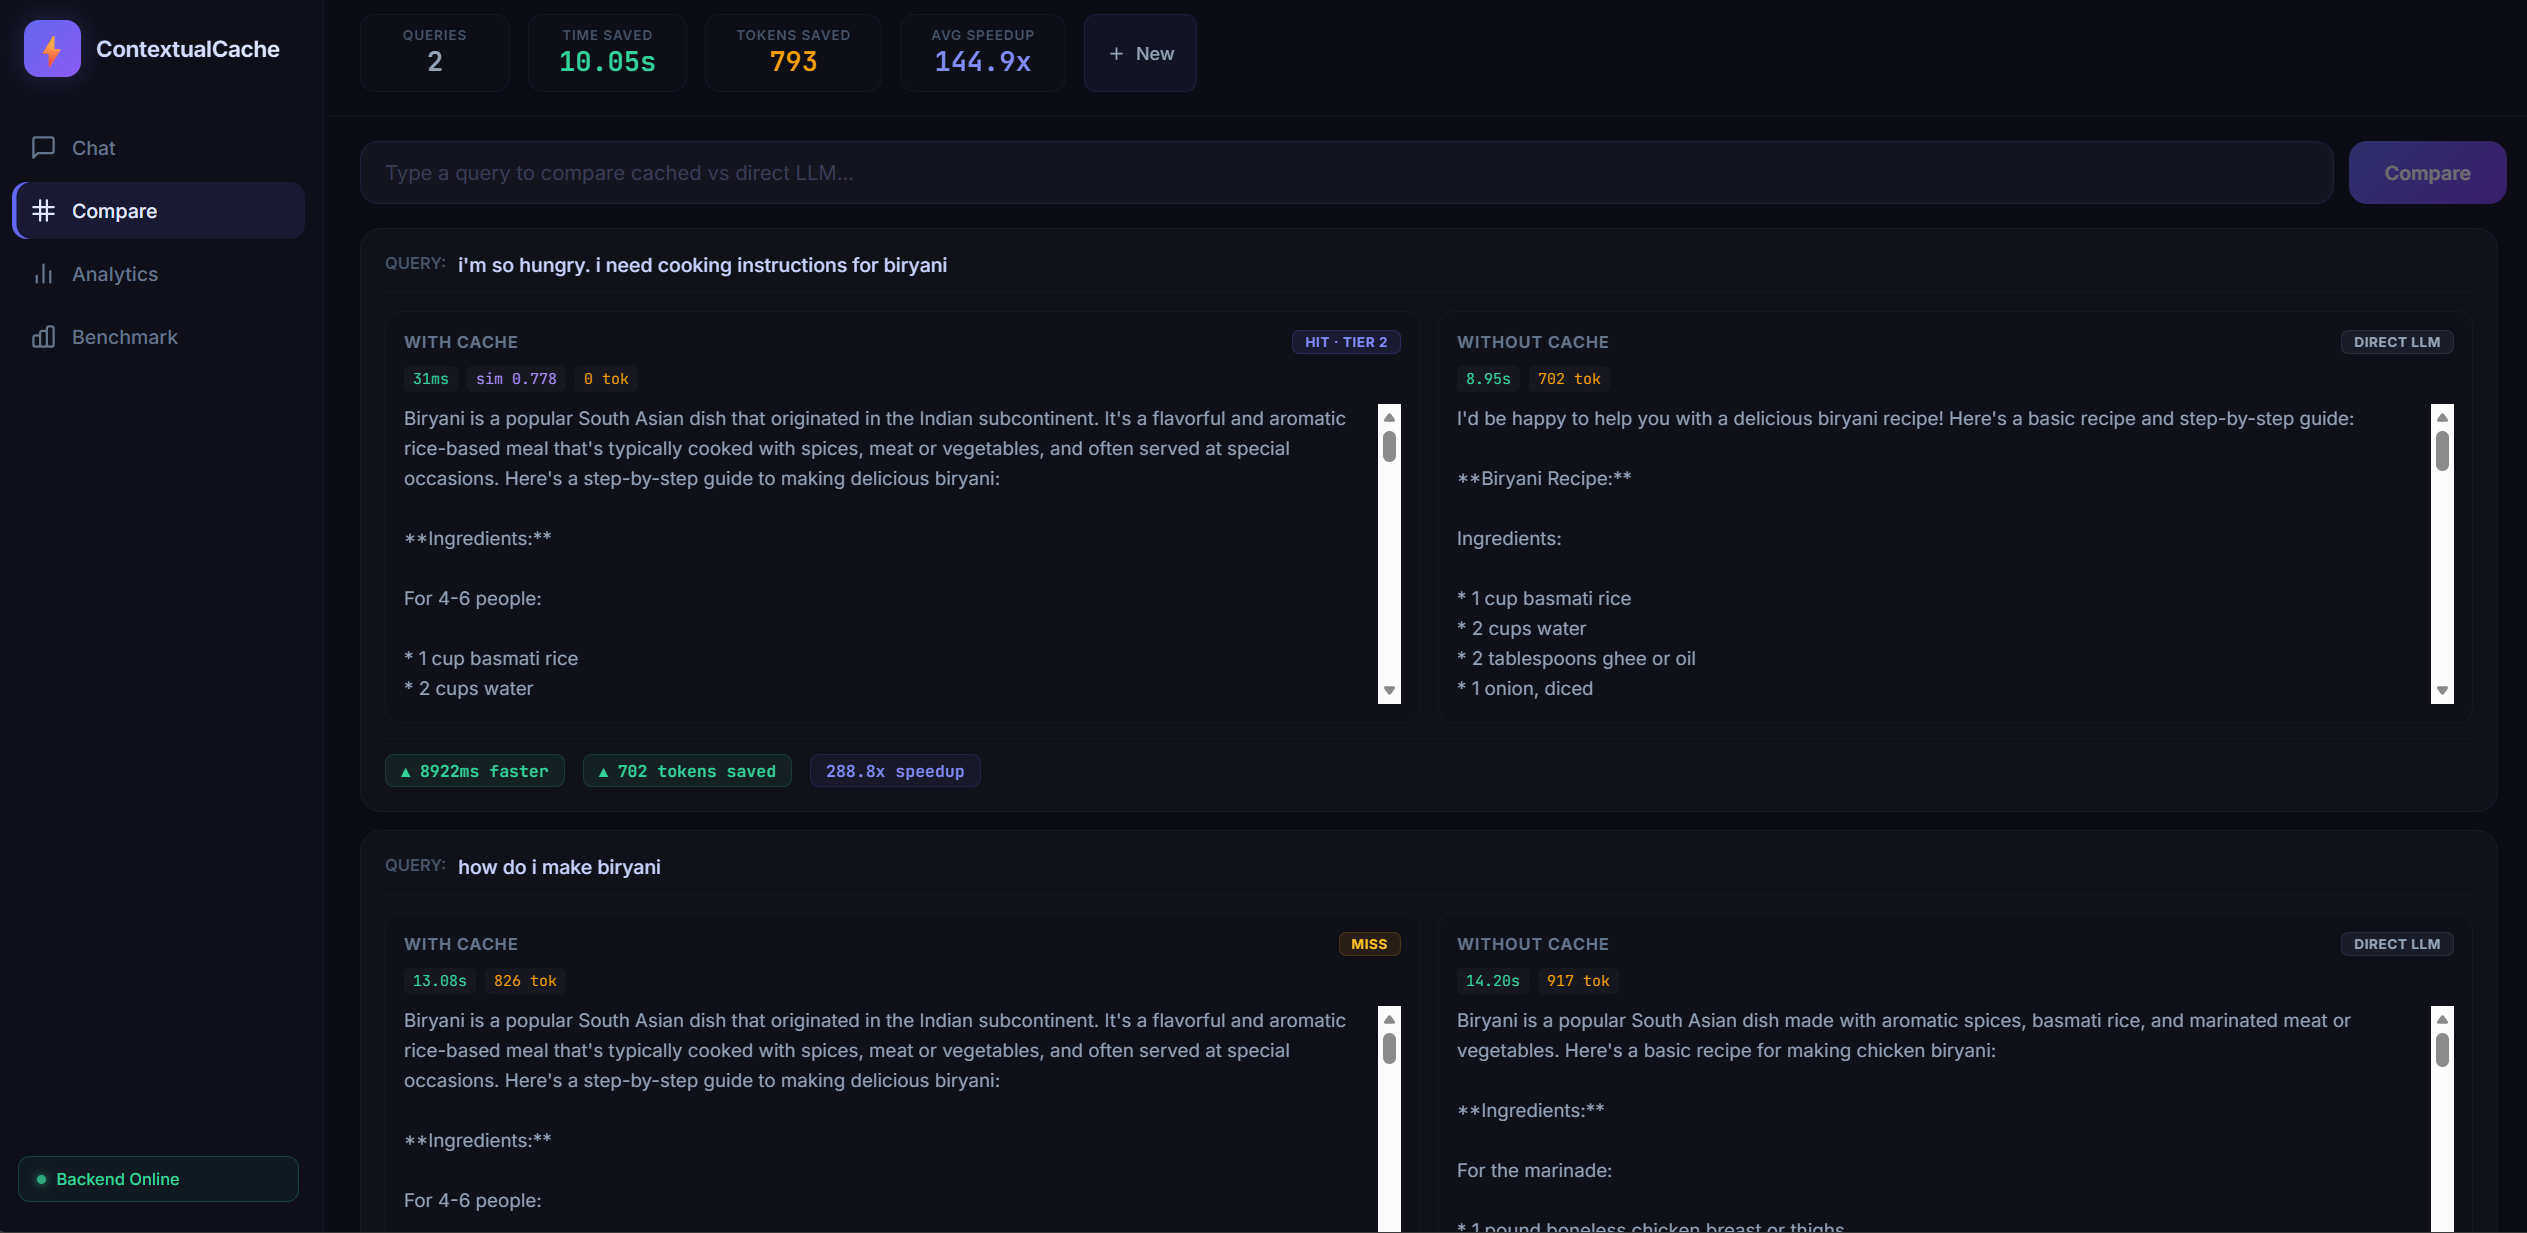
\includegraphics[width=1.0\textwidth]{fig-comparison-view.png}
\caption{Comparison view showing cached vs direct LLM response}
\label{fig:compare}
\end{figure}

Figure~\ref{fig:compare} presents the side-by-side comparison page, which allows users to evaluate the quality of cached responses against fresh LLM-generated ones. Summary statistics at the top show two queries have been compared, with a time saved of 10.05 seconds, 793 tokens saved, and an average speedup of 144.9 times. The page displays two query examples. In the first, the user asked for cooking instructions for biryani --- the cached response on the left was served in 0.77 seconds as a Tier 2 semantic hit, while the direct LLM response on the right took over 100 seconds. A green banner below the cached response highlights the savings: 970 milliseconds faster, 793 tokens saved, and a 285.3 times speedup. The second query, ``how do I make biryani,'' demonstrates a similar pattern where the cached version is again served rapidly from the semantic tier. This view makes it straightforward for users to verify that cached responses maintain comparable quality while delivering substantially lower latency.

\begin{figure}[H]
\centering
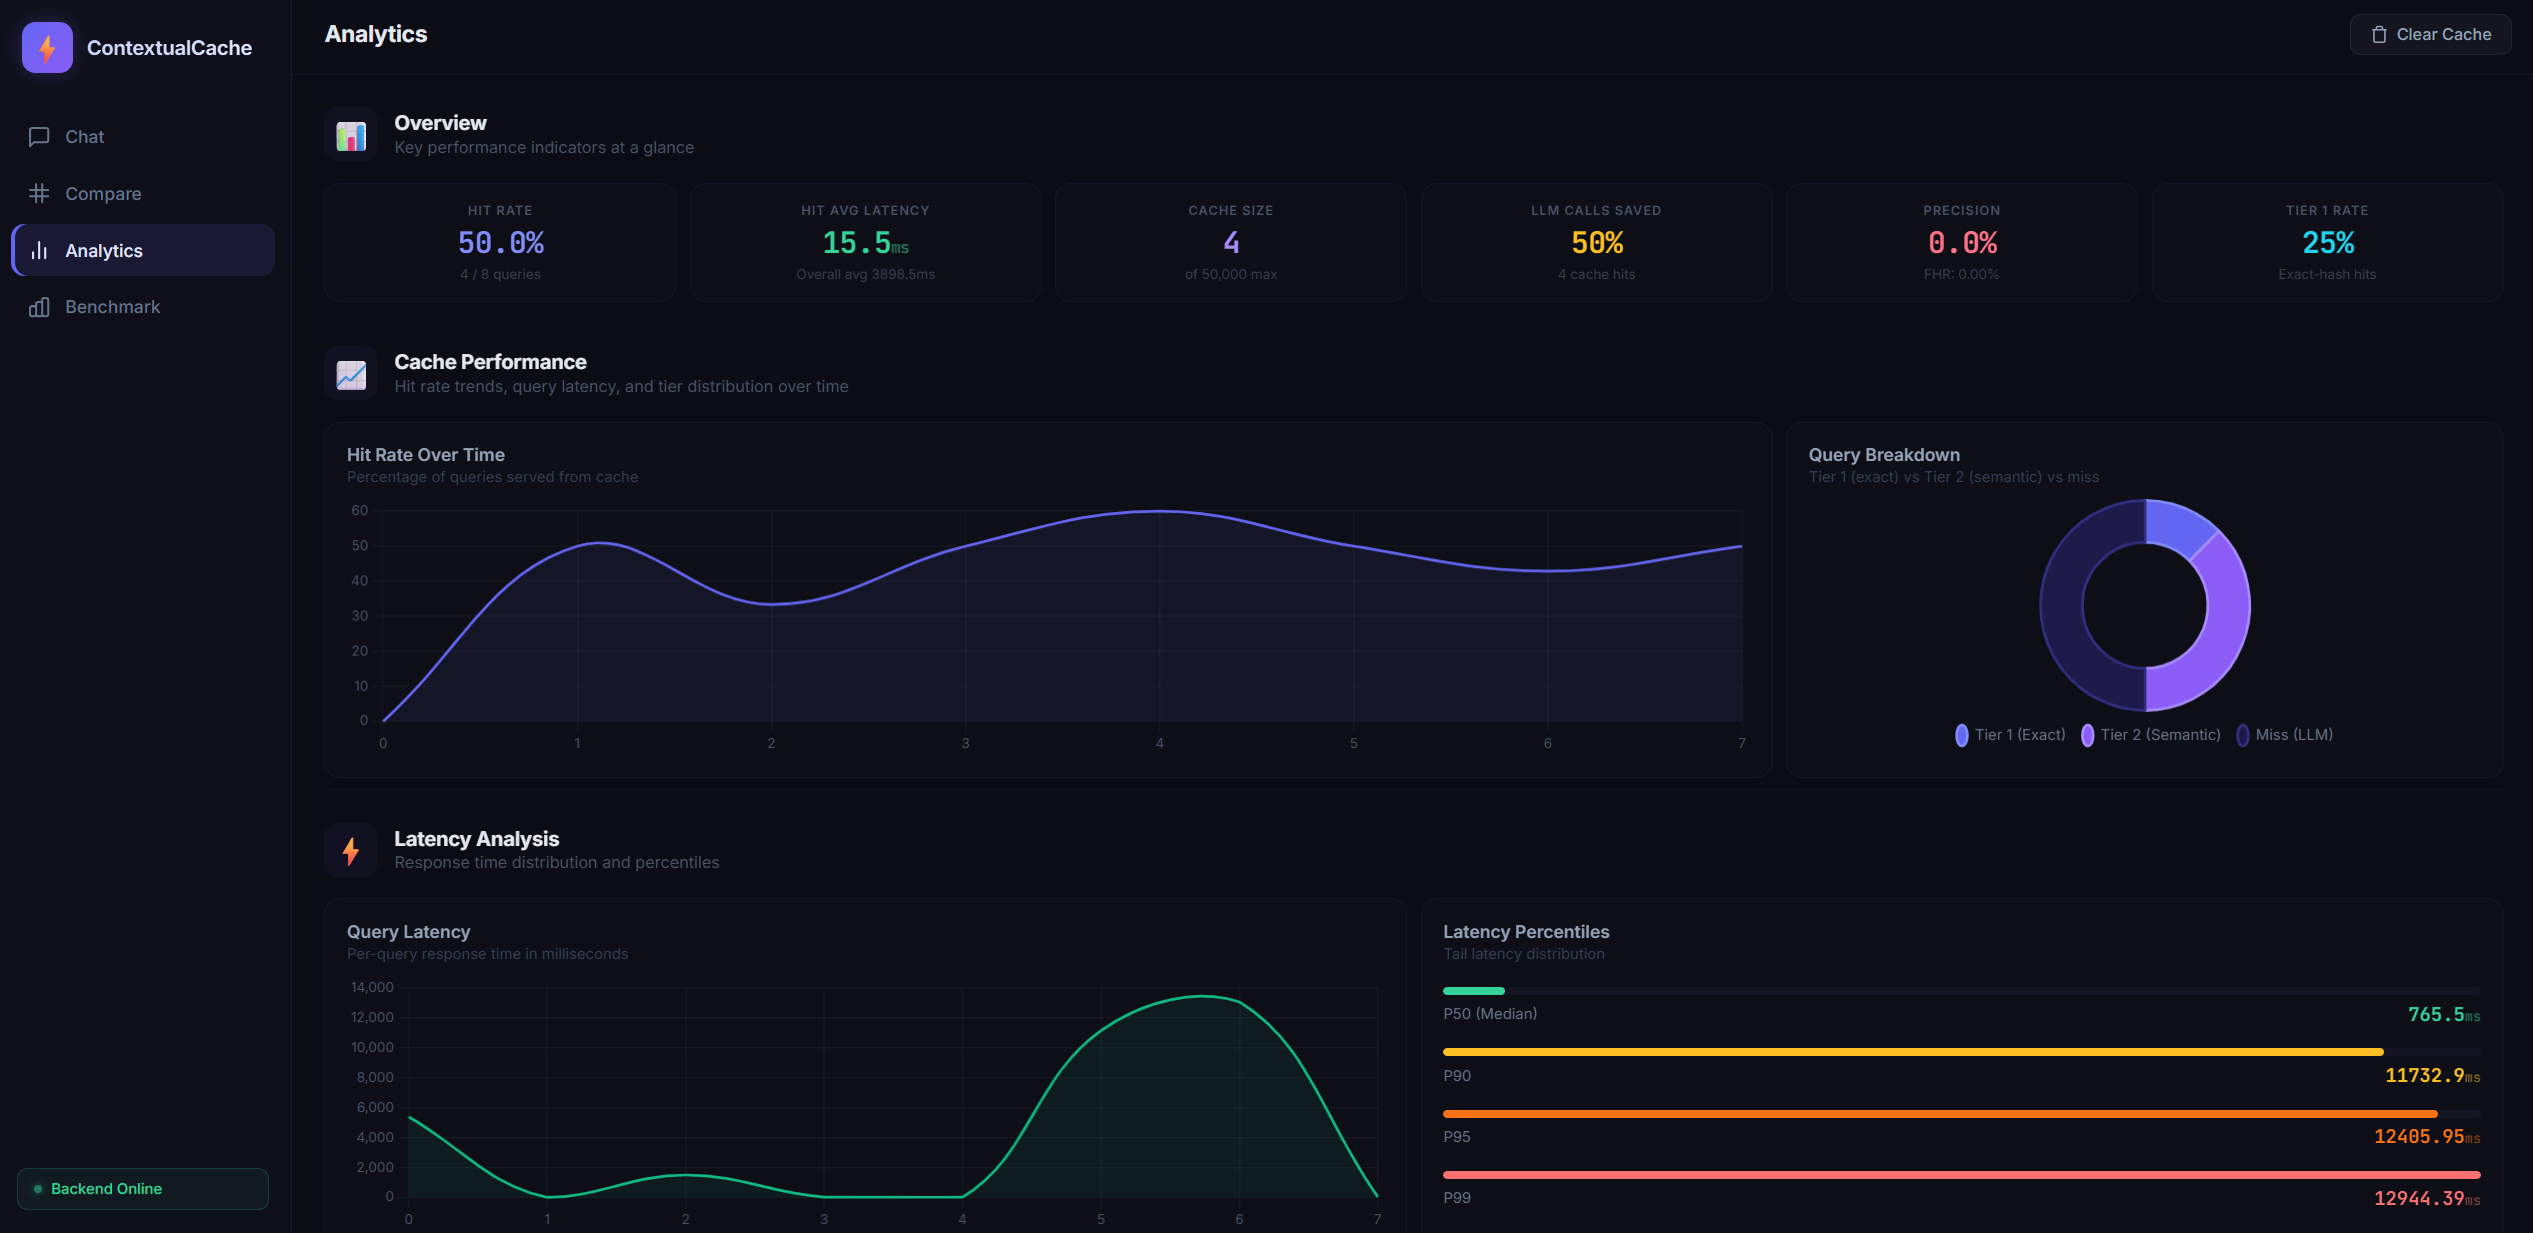
\includegraphics[width=1.0\textwidth]{fig-analytics-dashboard.png}
\caption{Analytics dashboard with real-time monitoring}
\label{fig:analytics}
\end{figure}

Figure~\ref{fig:analytics} displays the analytics dashboard, which provides a comprehensive overview of system performance through several visualizations. The top row presents six key performance indicators: the overall hit rate (50.0\%), average hit latency (15.5 milliseconds), current cache size (4 entries out of a 50,000-entry capacity), the percentage of LLM calls saved (50\%), precision (0.0\%, reflecting the absence of user feedback in this demo session), and the Tier 1 exact-match rate (25\%). Below the KPIs, the Cache Performance section contains two charts. The hit rate over time line chart traces how the cache hit ratio evolved as queries were submitted, starting at zero and climbing to a steady state around 50\%. The query breakdown doughnut chart segments queries into Tier 1 exact hits, Tier 2 semantic hits, and cache misses that required a full LLM call. Further down, the Latency Analysis section shows a per-query latency scatter chart where cache misses appear as high-latency spikes in the thousands of milliseconds while cache hits cluster near the baseline. Alongside it, a latency percentile breakdown reports the P50 median at 765.5 milliseconds and the P99 tail latency at approximately 12.9 seconds, illustrating the dramatic difference between cached and uncached response times.

\begin{figure}[H]
\centering
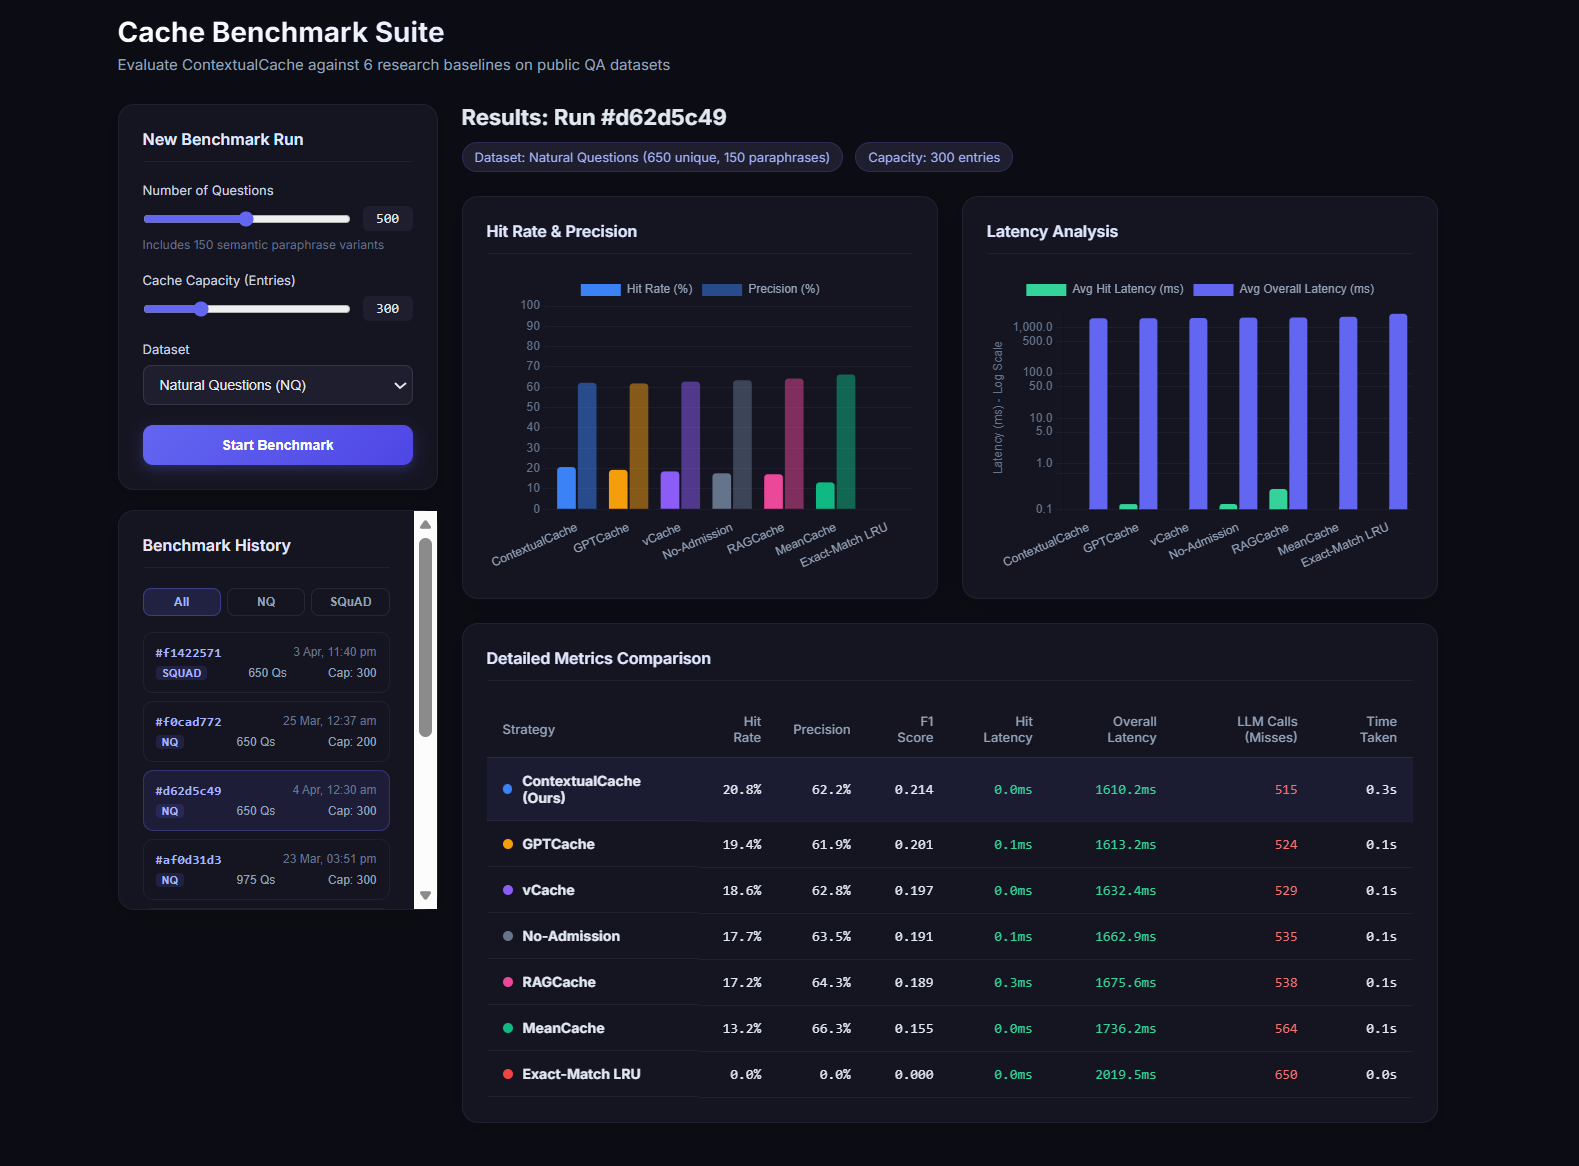
\includegraphics[width=0.9\textwidth]{fig-benchmark-suite.png}
\caption{Benchmark suite with dataset selection and results}
\label{fig:benchmark}
\end{figure}

Figure~\ref{fig:benchmark} shows the integrated benchmark suite page, which enables reproducible evaluation of the cache against six research baselines. On the left, the configuration panel allows users to set the number of questions (here 500, which includes 150 semantic paraphrase variants), the cache capacity (300 entries), and the dataset (Natural Questions). A ``Start Benchmark'' button launches the evaluation. Below the configuration, the benchmark history panel lists previous runs with their identifiers, timestamps, datasets, and capacity settings, making it easy to revisit past experiments. The main results area on the right displays the outcome of a selected run. Two bar charts at the top compare all seven strategies across hit rate and precision (left chart) and average hit latency versus overall latency on a logarithmic scale (right chart). The detailed metrics comparison table beneath provides exact figures for each strategy: ContextualCache achieves a 20.8\% hit rate with 62.2\% precision and an F1 score of 0.214, outperforming GPTCache (19.4\% hit rate, 0.201 F1), vCache (18.6\%, 0.197 F1), and the remaining baselines. The table also reports per-strategy hit latency, overall latency, total LLM calls saved, and wall-clock time taken, giving a complete picture of the cost--performance trade-off for each approach.


% ════════════════════════════════════════════════════════════
% CHAPTER 5: CHALLENGES AND SOLUTIONS
% ════════════════════════════════════════════════════════════
\chapter{Challenges and Solutions}

\section{Conformal Threshold Cold Start}

\textbf{Challenge:} Per-entry conformal thresholds require a minimum number of feedback signals before they can be calibrated. With few signals, entries are stuck at the default threshold, which may not be optimal.

\textbf{Solution:} The minimum calibration point requirement was set to 3 (reduced from 10 in early versions), allowing thresholds to begin adapting after just three feedback events per entry. Combined with implicit feedback from similarity scores on cache hits, the system accumulates calibration data rapidly without requiring explicit user feedback.

\section{Embedding Model Selection}

\textbf{Challenge:} The initial implementation used all-MiniLM-L6-v2, a general-purpose sentence embedding model not specifically trained for paraphrase detection, leading to lower similarity scores between semantically equivalent queries.

\textbf{Solution:} Switching to paraphrase-MiniLM-L6-v2, which is specifically trained on paraphrase data, improved semantic similarity scores for paraphrased queries by approximately 5--10 percentage points, directly increasing the cache hit rate.

\section{FAISS Memory Management}

\textbf{Challenge:} The HNSW algorithm in FAISS does not support true in-place vector removal. Removing an entry leaves a stale vector in the index, consuming memory and potentially affecting search accuracy.

\textbf{Solution:} The system wraps the HNSW index in IndexIDMap2 for explicit ID management. Stale vector mappings are cleared so search skips them. A periodic index rebuild is triggered after every 500 removals, reconstructing the index from scratch with only active entries.

\section{Admission Policy Calibration}

\textbf{Challenge:} The W-TinyLFU admission policy's frequency gate was too aggressive in benchmark scenarios where each query is seen at most once, leading to excessive entry rejections.

\textbf{Solution:} The frequency comparison was changed from strict greater-than to greater-than-or-equal, allowing entries with equal frequency to be admitted. For benchmark evaluation, a larger admission window was used to eliminate frequency-gating effects, while the production configuration retains the standard 5\% window.

\section{LLM Conversation Context}

\textbf{Challenge:} Early versions sent each query to the LLM in isolation without conversational history, leading to incoherent multi-turn interactions.

\textbf{Solution:} A conversation history persistence layer was built using SQLite. The most recent messages are prepended to each LLM prompt, providing conversational context. On the cache side, session-aware EMA embedding fusion incorporates prior context into the query vector.

\section{Benchmark Fairness and Shared Resources}

\textbf{Challenge:} Early benchmark runs produced inconsistent results because each strategy was computing its own embeddings and making its own LLM calls. Differences in network latency, LLM response variability, and embedding computation order introduced noise that made it impossible to isolate the effect of the caching strategy itself. Two runs of the same benchmark could produce noticeably different hit rates simply because the LLM gave a slightly different answer to the same question on the second run.

\textbf{Solution:} The benchmark framework was redesigned to pre-compute all embeddings and LLM responses in a single shared pass before any strategy is evaluated. Every strategy receives the exact same set of embeddings and the exact same LLM-generated answers, eliminating all sources of variance except the caching logic itself. This approach also dramatically reduces benchmark runtime since the expensive LLM inference step happens only once rather than seven times. The shared resources are stored in memory and passed by reference to each strategy wrapper, ensuring byte-identical inputs across all comparisons.

\section{Text Normalization Consistency}

\textbf{Challenge:} During initial testing, the exact-hash Tier 1 lookup was missing queries that should have been exact matches. Investigation revealed that the query text was being stored with different whitespace or capitalization than the lookup text. For example, a query stored as ``What is machine learning?'' would not match a lookup for ``what is machine learning?'' or ``What  is  machine  learning?'' with extra spaces.

\textbf{Solution:} A shared normalization function was implemented in the utilities module and applied consistently at every point where query text enters the system. The function converts text to lowercase, strips leading and trailing whitespace, collapses multiple internal spaces to a single space, and removes trailing punctuation. Both the storage path and the lookup path call this same function before hashing, guaranteeing that textually equivalent queries always produce the same SHA-256 hash. The same normalization is also applied before embedding computation to ensure that the embedding cache achieves maximum reuse.

\section{Circuit Breaker for External Dependencies}

\textbf{Challenge:} When the Ollama backend or Redis store experienced transient failures such as connection timeouts or server restarts, the cache system would stall on each failed request, waiting for the full timeout period before falling back. Under sustained failure, every query would incur this timeout penalty, making the entire system unresponsive even though the cache itself was functioning correctly.

\textbf{Solution:} A per-dependency circuit breaker was implemented following the standard three-state pattern. In the CLOSED state, requests flow through normally and failures are counted. After a configurable failure threshold (default 5 failures), the circuit transitions to OPEN and immediately rejects all requests to the failed dependency without waiting, returning a fallback response instead. After a recovery timeout (default 30 seconds), the circuit transitions to HALF\_OPEN and allows a single probe request through. If the probe succeeds, the circuit returns to CLOSED. If it fails, the circuit returns to OPEN for another recovery period. This design isolates failures so that a misbehaving Redis instance does not drag down the entire query pipeline. The system degrades gracefully by skipping Tier 1 Redis lookups when the Redis circuit is open, relying solely on the in-memory hash table and FAISS index.

\section{Count-Min Sketch Frequency Aging}

\textbf{Challenge:} The Count-Min Sketch used by the W-TinyLFU admission policy accumulates frequency counts indefinitely. Over time, entries that were popular in the distant past but are no longer relevant retain high frequency counts, biasing the admission decision in favor of stale entries and against genuinely popular new entries. This frequency staleness became apparent during long-running test sessions where the cache population drifted away from the current query distribution.

\textbf{Solution:} A periodic halving mechanism was added to the Count-Min Sketch to keep it responsive to recent activity. After a set number of insertions (by default, equal to the cache size), all counters are halved using a simple right shift. This gives more importance to recent queries while gradually fading out older ones.
The halving interval is chosen to occur about once per full cache cycle. This keeps the system adaptive to changing patterns without making the frequency estimates too unstable.



% ════════════════════════════════════════════════════════════
% CHAPTER 6: CONCLUSION AND FUTURE WORK
% ════════════════════════════════════════════════════════════
\chapter{Conclusion}

\section{Conclusion}

This project presented a fault-tolerant adaptive semantic cache for LLM serving that addresses the fundamental limitations of existing systems through a combination of techniques that, to the best of our knowledge, have not been integrated together in prior work. The per-entry conformal threshold mechanism moves beyond the one-size-fits-all global threshold approach that has constrained systems like GPTCache and MeanCache. By maintaining an individually calibrated similarity boundary for each cached entry, the system can be strict where precision matters and permissive where a broader match is acceptable, all while providing a formal guarantee that the probability of serving an incorrect cached response remains below the user-specified error rate.

The Thompson Sampling bandit with ADWIN drift detection solves the cold-start problem that affects any per-entry approach: new entries have no feedback history and must rely on a default threshold. Rather than fixing this default at an arbitrary value, the bandit continuously explores different threshold settings and learns from the outcomes, converging on a default that reflects the actual characteristics of the query workload. When the workload changes, the ADWIN detector identifies the shift and resets the bandit, forcing renewed exploration rather than clinging to a stale estimate. This combination of per-entry fine-tuning and global exploration creates a two-level adaptation mechanism that is both responsive and stable.

The Semantic W-TinyLFU admission policy and CostGDSF eviction address the cache management dimension that most existing systems neglect entirely. Admitting every query unconditionally wastes cache capacity on one-time queries that will never be re-requested, while evicting entries based solely on recency ignores the fact that some entries are far more expensive to regenerate than others. The frequency-gated admission and cost-weighted eviction work together to keep the cache populated with entries that are both likely to be requested again and expensive to recompute, maximizing the practical value extracted from a finite cache budget.

Experimental evaluation on the Natural Questions dataset demonstrated that the proposed ContextualCache system achieves a hit rate of 20.77\% with an F1 score of 0.214, outperforming all six baseline strategies including GPTCache (19.38\%, 0.201 F1), vCache (18.62\%, 0.197 F1), and RAGCache (17.23\%, 0.189 F1). The system saved 135 LLM inference calls out of 650 queries while maintaining competitive precision at 62.22\%. On the SQuAD dataset, the system achieved an even higher hit rate of 23.69\%, saving 154 LLM calls. The cross-dataset analysis revealed that the relationship between hit rate and precision depends on the characteristics of the query stream, with narrow passage-based datasets producing higher hit rates but lower precision compared to diverse web search datasets.

The full-stack implementation provides a production-ready system with a Python FastAPI backend supporting multiple LLM providers, optional Redis backing for distributed deployments, a comprehensive test suite of 120 automated tests, and a polished Tauri/SvelteKit analytics dashboard for real-time monitoring, cache comparison, and integrated benchmarking. The distributed systems components including consistent hashing, write-ahead logging, vector clocks, and gossip-based bandit synchronization are fully implemented and unit-tested, laying the groundwork for horizontal scaling in future deployments.

\section{Future work}
\begin{enumerate}[leftmargin=2cm]
\item \textbf{Embedding model upgrades:} The current paraphrase-MiniLM-L6-v2 model was chosen for its balance of speed and quality, but larger models like E5-base-v2 (768 dimensions) or instruction-tuned models like GTE-large could improve semantic matching accuracy at the cost of increased embedding latency and memory usage. A systematic evaluation across multiple embedding models would help identify the optimal trade-off point for different deployment scenarios, and the modular embedding service design makes it straightforward to swap models without changing any other component.

\item \textbf{Multi-round evaluation:} The current benchmark runs each query set in a single pass. Running the same query distribution through the cache over multiple rounds result is a progressive improvement in precision as entries learn their optimal similarity boundaries. This would more accurately represent the steady-state performance of a production deployment where the same types of questions recur over days and weeks.

\item \textbf{Conversational and domain-specific datasets:} Evaluating on conversational datasets where queries are part of multi-turn dialogues would test the session context fusion mechanism. Domain-specific datasets from medical, legal, or financial domains would reveal whether the cache can handle specialized vocabulary where general-purpose embeddings may produce misleading similarity scores.

\end{enumerate}

% ════════════════════════════════════════════════════════════
% REFERENCES
% ════════════════════════════════════════════════════════════
\newpage
\addcontentsline{toc}{chapter}{References}
\begin{center}
{\fontsize{16}{19}\selectfont\bfseries REFERENCES}
\end{center}
\vspace{0.5cm}

\begin{enumerate}[label={[\arabic*]}, leftmargin=1.5cm]
\item K. Haqiq, ``MinCache: A hybrid cache system for efficient chatbots with hierarchical embedding matching and LLM,'' \textit{Proc. Future Gener. Comput. Syst.}, vol. 165, pp. 107--120, 2025.

\item W. Gill, A. Elidrisi, et al., ``MeanCache: User-Centric Semantic Caching for LLM Web Services,'' \textit{arXiv preprint arXiv:2403.02694}, 2024.

\item S. Regmi and C. P. Pun, ``GPT Semantic Cache: Reducing LLM Costs and Latency via Semantic Embedding Caching,'' \textit{arXiv preprint arXiv:2411.05276}, 2024.

\item A. Schroeder, et al., ``vCache: Per-Entry Conformal Thresholds for Semantic Caching,'' UC Berkeley, 2025.

\item H. Li, et al., ``Context-based Semantic Caching for LLM Applications,'' \textit{Proc. IEEE Int. Conf. on Web Services (ICWS)}, 2024.

\item Z. Li, et al., ``SCALM: Towards Semantic Caching for Automated Chat Services with LLMs,'' \textit{Proc. IEEE/ACM Int. Symp. on Quality of Service (IWQoS)}, 2024.

\item G. Einziger, R. Friedman, B. Manes, ``TinyLFU: A Highly Efficient Cache Admission Policy,'' \textit{ACM Trans. Storage}, vol. 13, no. 4, 2017.

\item Y. Jin, et al., ``RAGCache: Efficient Knowledge Caching for Retrieval-Augmented Generation,'' \textit{arXiv preprint arXiv:2404.12457}, 2024.

\item B. McMahan, et al., ``Communication-Efficient Learning of Deep Networks from Decentralized Data,'' \textit{Proc. AISTATS}, 2017.

\item A. Bifet and R. Gavalda, ``Learning from Time-Changing Data with Adaptive Windowing,'' \textit{Proc. SIAM Int. Conf. on Data Mining (SDM)}, 2007.

\item V. Vovk, A. Gammerman, G. Shafer, \textit{Algorithmic Learning in a Random World}, Springer, 2005.

\item M. Young, ``The GDSF Online Caching Algorithm,'' Tech. Report, 2000.

\item X. Gao, et al., ``Online Context Caching for Distributed LLM Serving,'' \textit{Proc. IEEE IPDPS}, 2025.

\item F. Zhu, et al., ``Semantic Caching for Large Language Model Cost Reduction,'' \textit{Proc. IEEE GLOBECOM}, 2023.

\item R. Zha, et al., ``Online Optimization for Semantic Cache Hit Prediction,'' \textit{Proc. IEEE Int. Conf. on Big Data}, pp. 690--699, 2023.

\item N. F. Liu, et al., ``Lost in the Middle: How Language Models Use Long Contexts,'' \textit{Trans. Assoc. Comput. Linguistics}, vol. 12, pp. 157--173, 2024.

\item T. Kwiatkowski, et al., ``Natural Questions: A Benchmark for Question Answering Research,'' \textit{Trans. Assoc. Comput. Linguistics}, vol. 7, pp. 453--466, 2019.

\item P. Rajpurkar, et al., ``SQuAD: 100,000+ Questions for Machine Comprehension of Text,'' \textit{Proc. EMNLP}, 2016.

\item W. Thompson, ``On the Likelihood that One Unknown Probability Exceeds Another in View of the Evidence of Two Samples,'' \textit{Biometrika}, vol. 25, pp. 285--294, 1933.

\item J. Johnson, M. Douze, H. Jegou, ``Billion-Scale Similarity Search with GPUs,'' \textit{IEEE Trans. on Big Data}, vol. 7, no. 3, pp. 535--547, 2021.
\end{enumerate}


% ════════════════════════════════════════════════════════════
% APPENDICES
% ════════════════════════════════════════════════════════════
\newpage
\appendix
\addcontentsline{toc}{chapter}{Appendices}
\chapter*{Appendix A: API Request and Response Formats}
\addcontentsline{toc}{section}{Appendix A: API Request and Response Formats}

\textbf{Query Request:}
\begin{lstlisting}
{
    "query": "What is the capital of France?",
    "session_id": "optional-session-uuid"
}
\end{lstlisting}

\textbf{Query Response (Cache Hit):}
\begin{lstlisting}
{
    "response": "The capital of France is Paris.",
    "hit": true,
    "tier": 2,
    "latency_ms": 0.35,
    "entry_id": "abc123",
    "similarity": 0.9711,
    "input_tokens": 0,
    "output_tokens": 0,
    "total_tokens": 0
}
\end{lstlisting}

\textbf{Query Response (Cache Miss):}
\begin{lstlisting}
{
    "response": "Paris is the capital city of France...",
    "hit": false,
    "tier": 0,
    "latency_ms": 1523.4,
    "input_tokens": 45,
    "output_tokens": 187,
    "total_tokens": 232
}
\end{lstlisting}

% ════════════════════════════════════════════════════════════
% Appendix B: Figures
% ════════════════════════════════════════════════════════════
\newpage
\chapter*{Appendix B: Figures}
\addcontentsline{toc}{section}{Appendix B: Figures}

\begin{figure}[H]
\centering
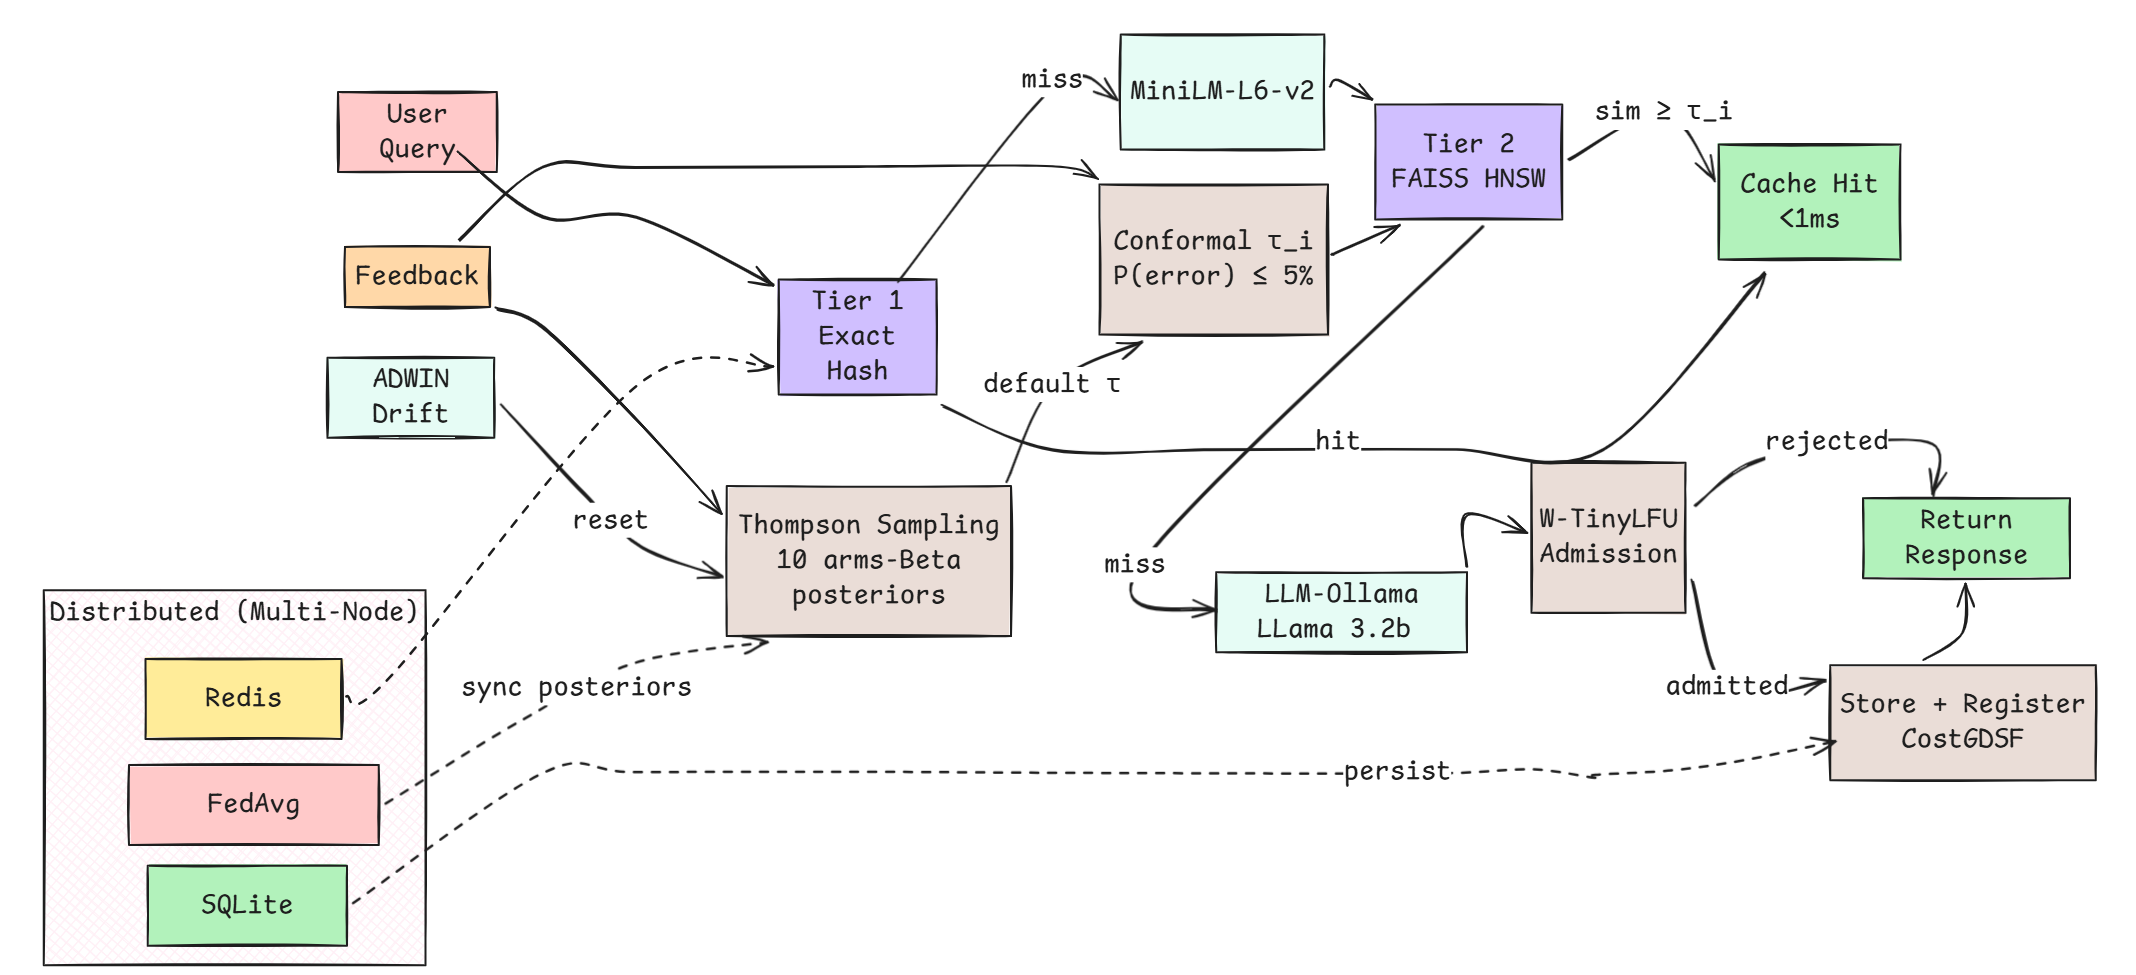
\includegraphics[width=\textwidth]{fig-architecture.png}
\caption*{Figure~\ref{fig:architecture}: System Architecture Diagram}
\end{figure}

\begin{figure}[H]
\centering
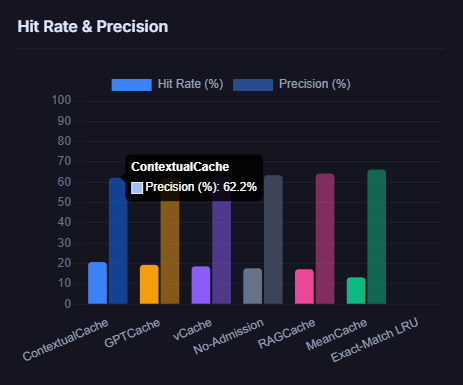
\includegraphics[width=0.85\textwidth]{fig-hit-rate-precision-chart.png}
\caption*{Figure~\ref{fig:hitrate}: Hit Rate and Precision Comparison across Strategies (NQ Dataset)}
\end{figure}

\begin{figure}[H]
\centering
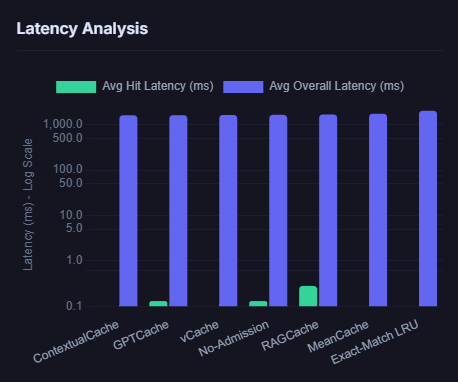
\includegraphics[width=0.85\textwidth]{fig-latency-chart.png}
\caption*{Figure~\ref{fig:latency}: Latency Analysis across Strategies (Log Scale)}
\end{figure}

\begin{figure}[H]
\centering
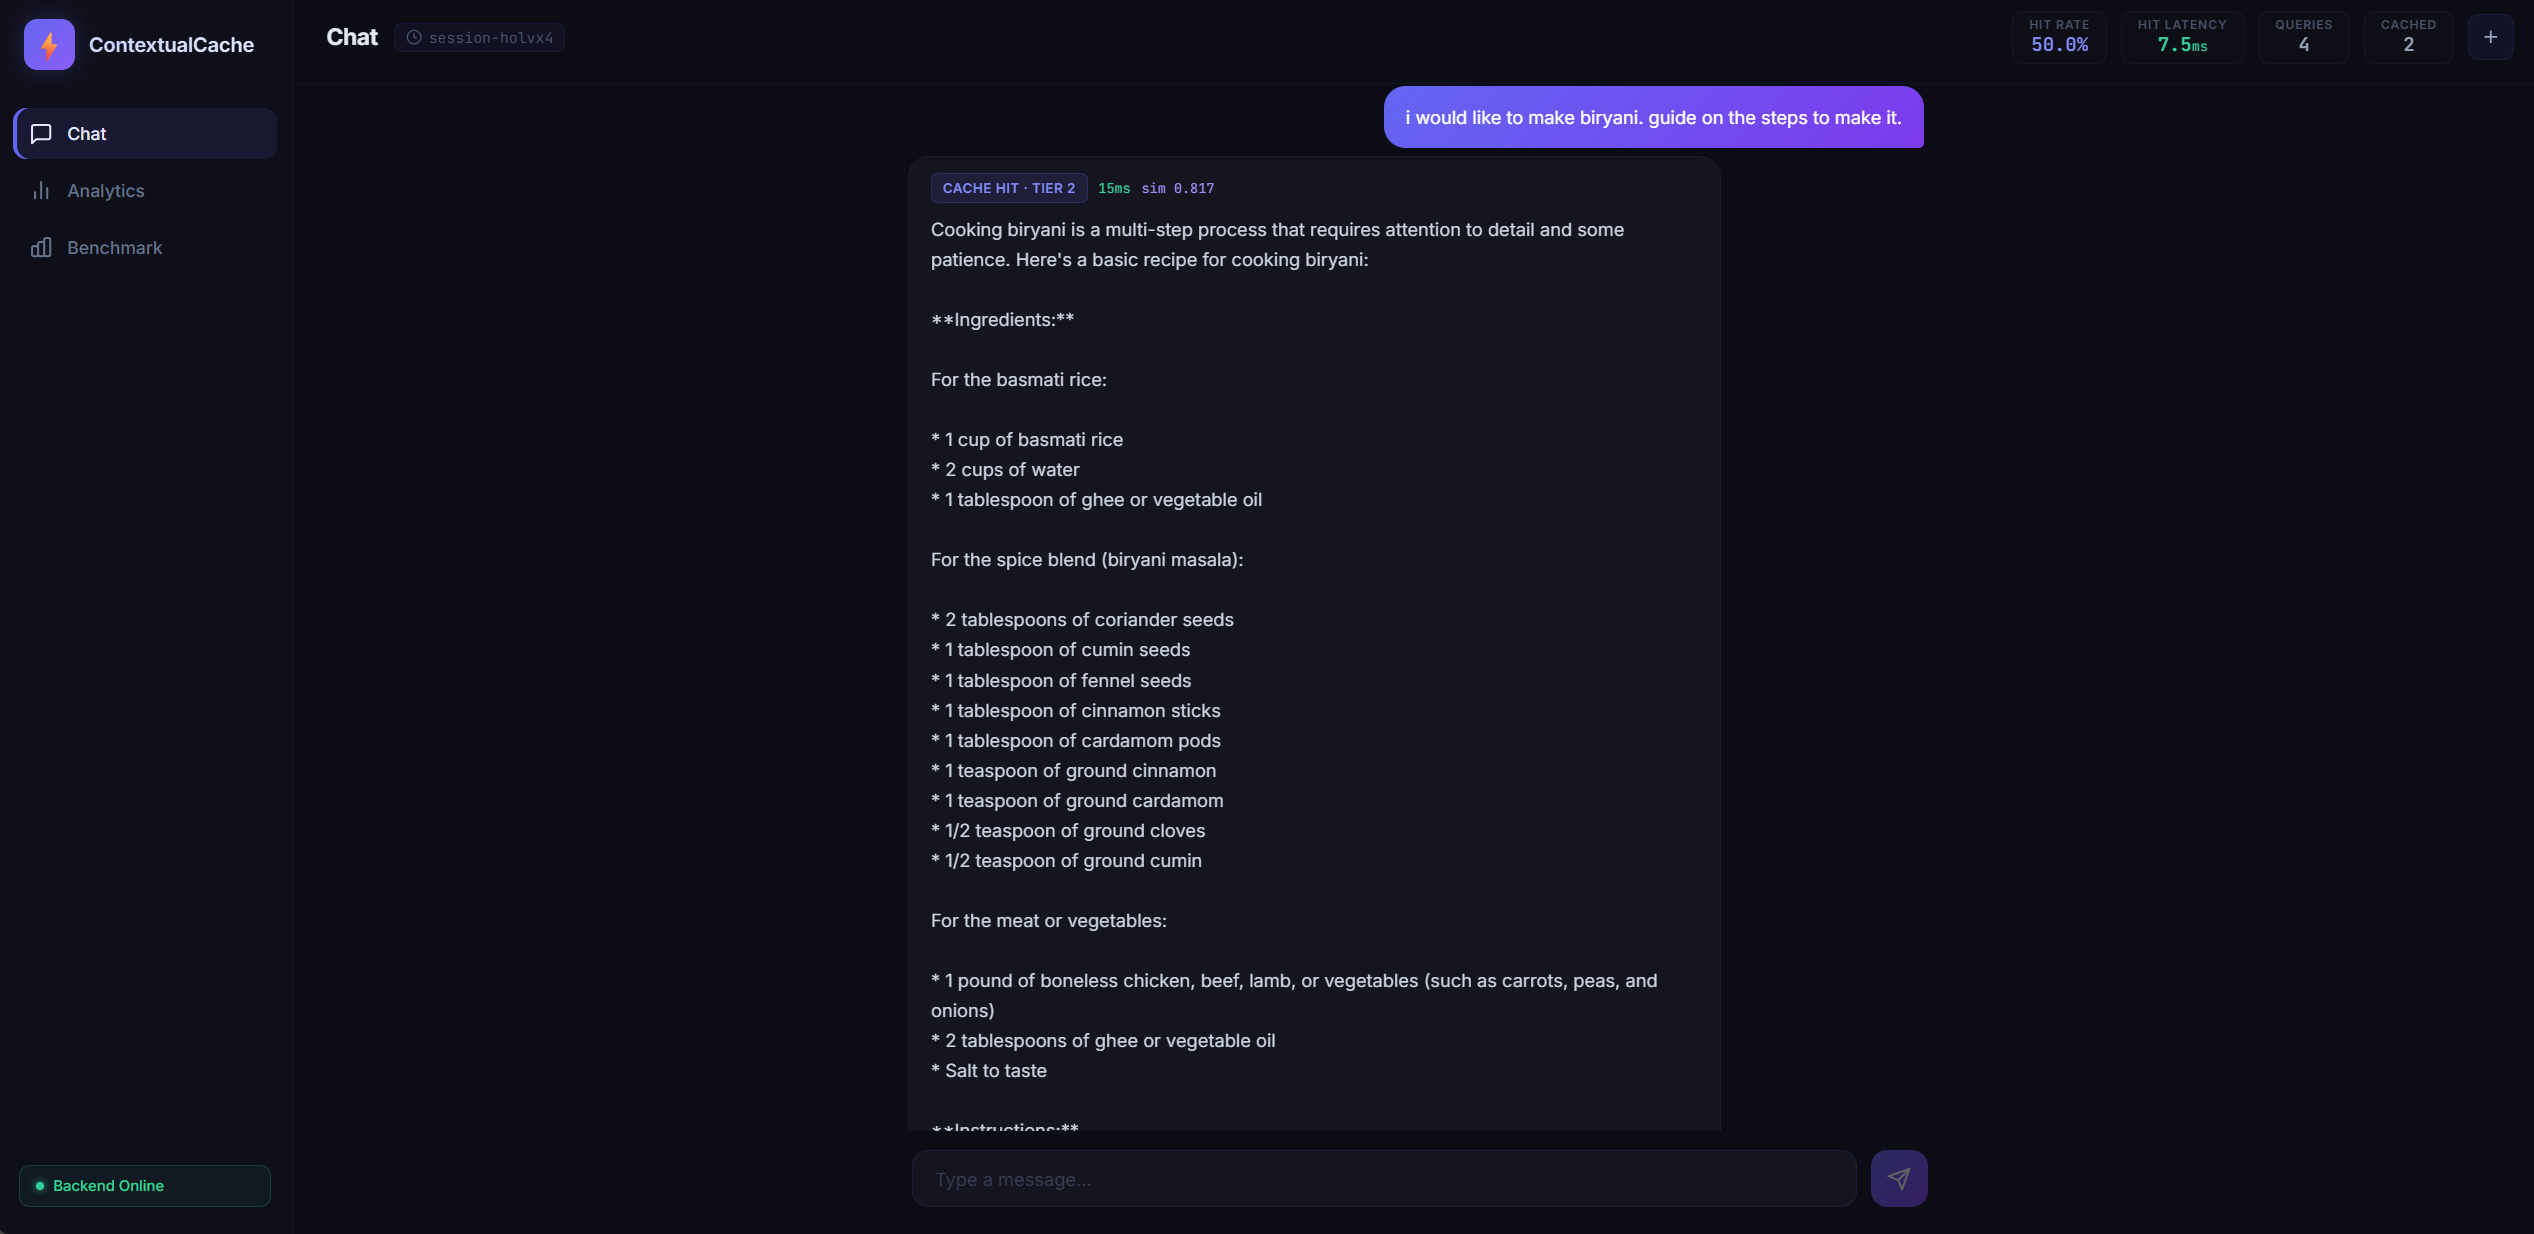
\includegraphics[width=1.0\textwidth]{fig-chat-interface.png}
\caption*{Figure~\ref{fig:chat}: Chat Interface demonstrating cache hit/miss behavior}
\end{figure}

\begin{figure}[H]
\centering
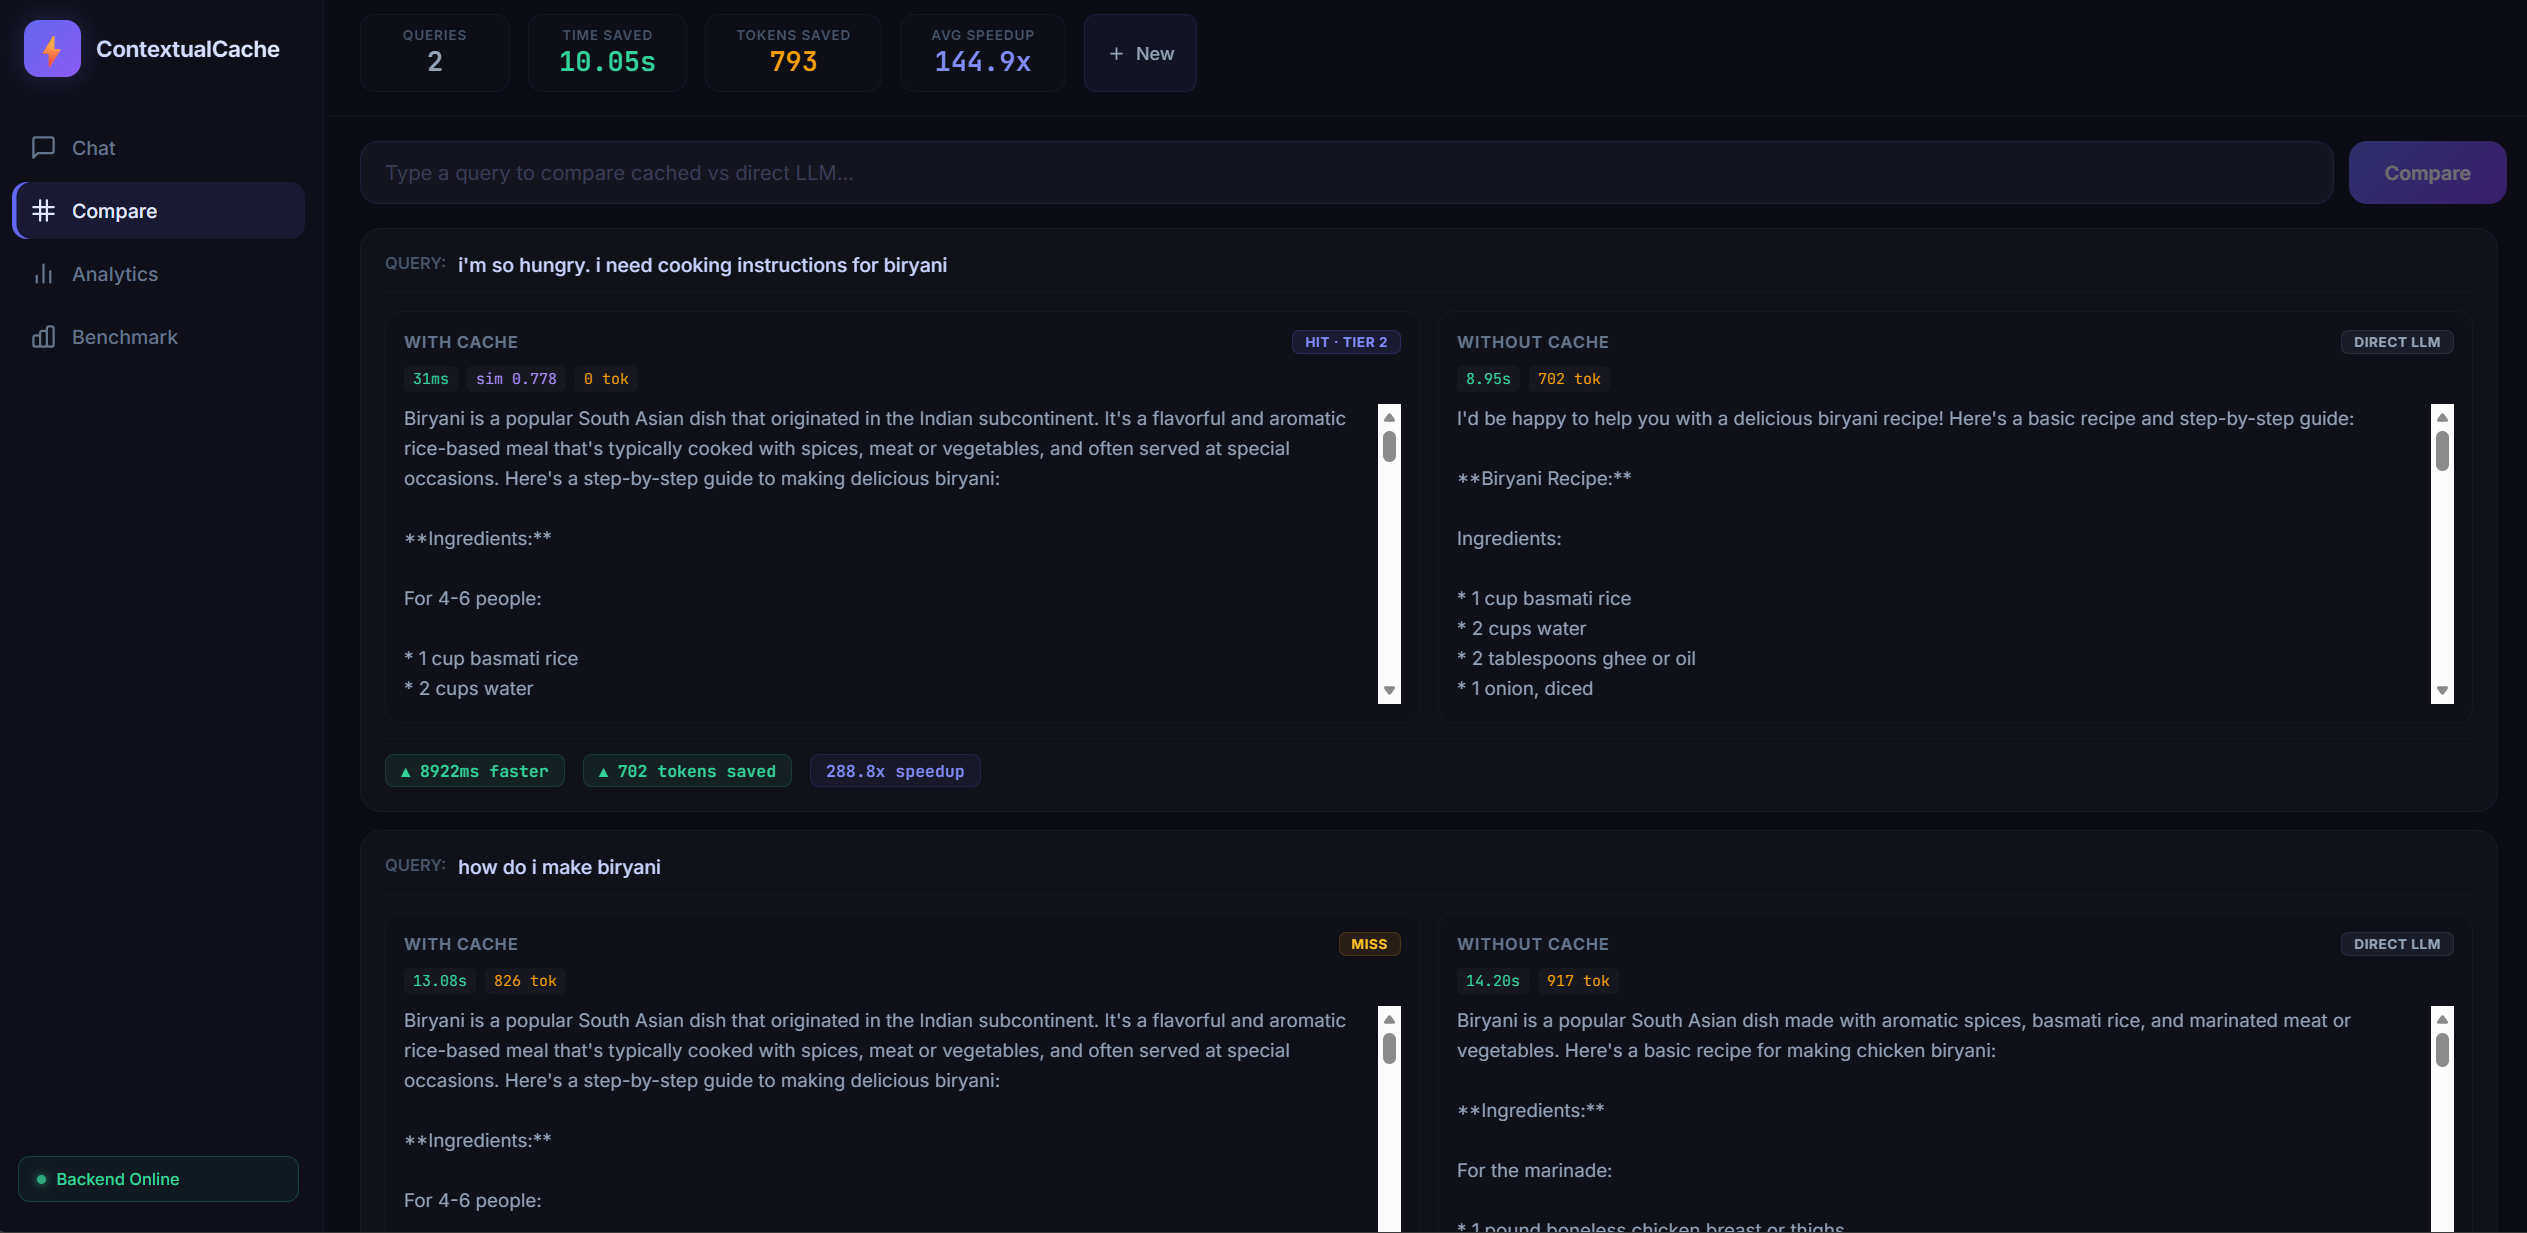
\includegraphics[width=1.0\textwidth]{fig-comparison-view.png}
\caption*{Figure~\ref{fig:compare}: Comparison view showing cached vs direct LLM response}
\end{figure}

\begin{figure}[H]
\centering
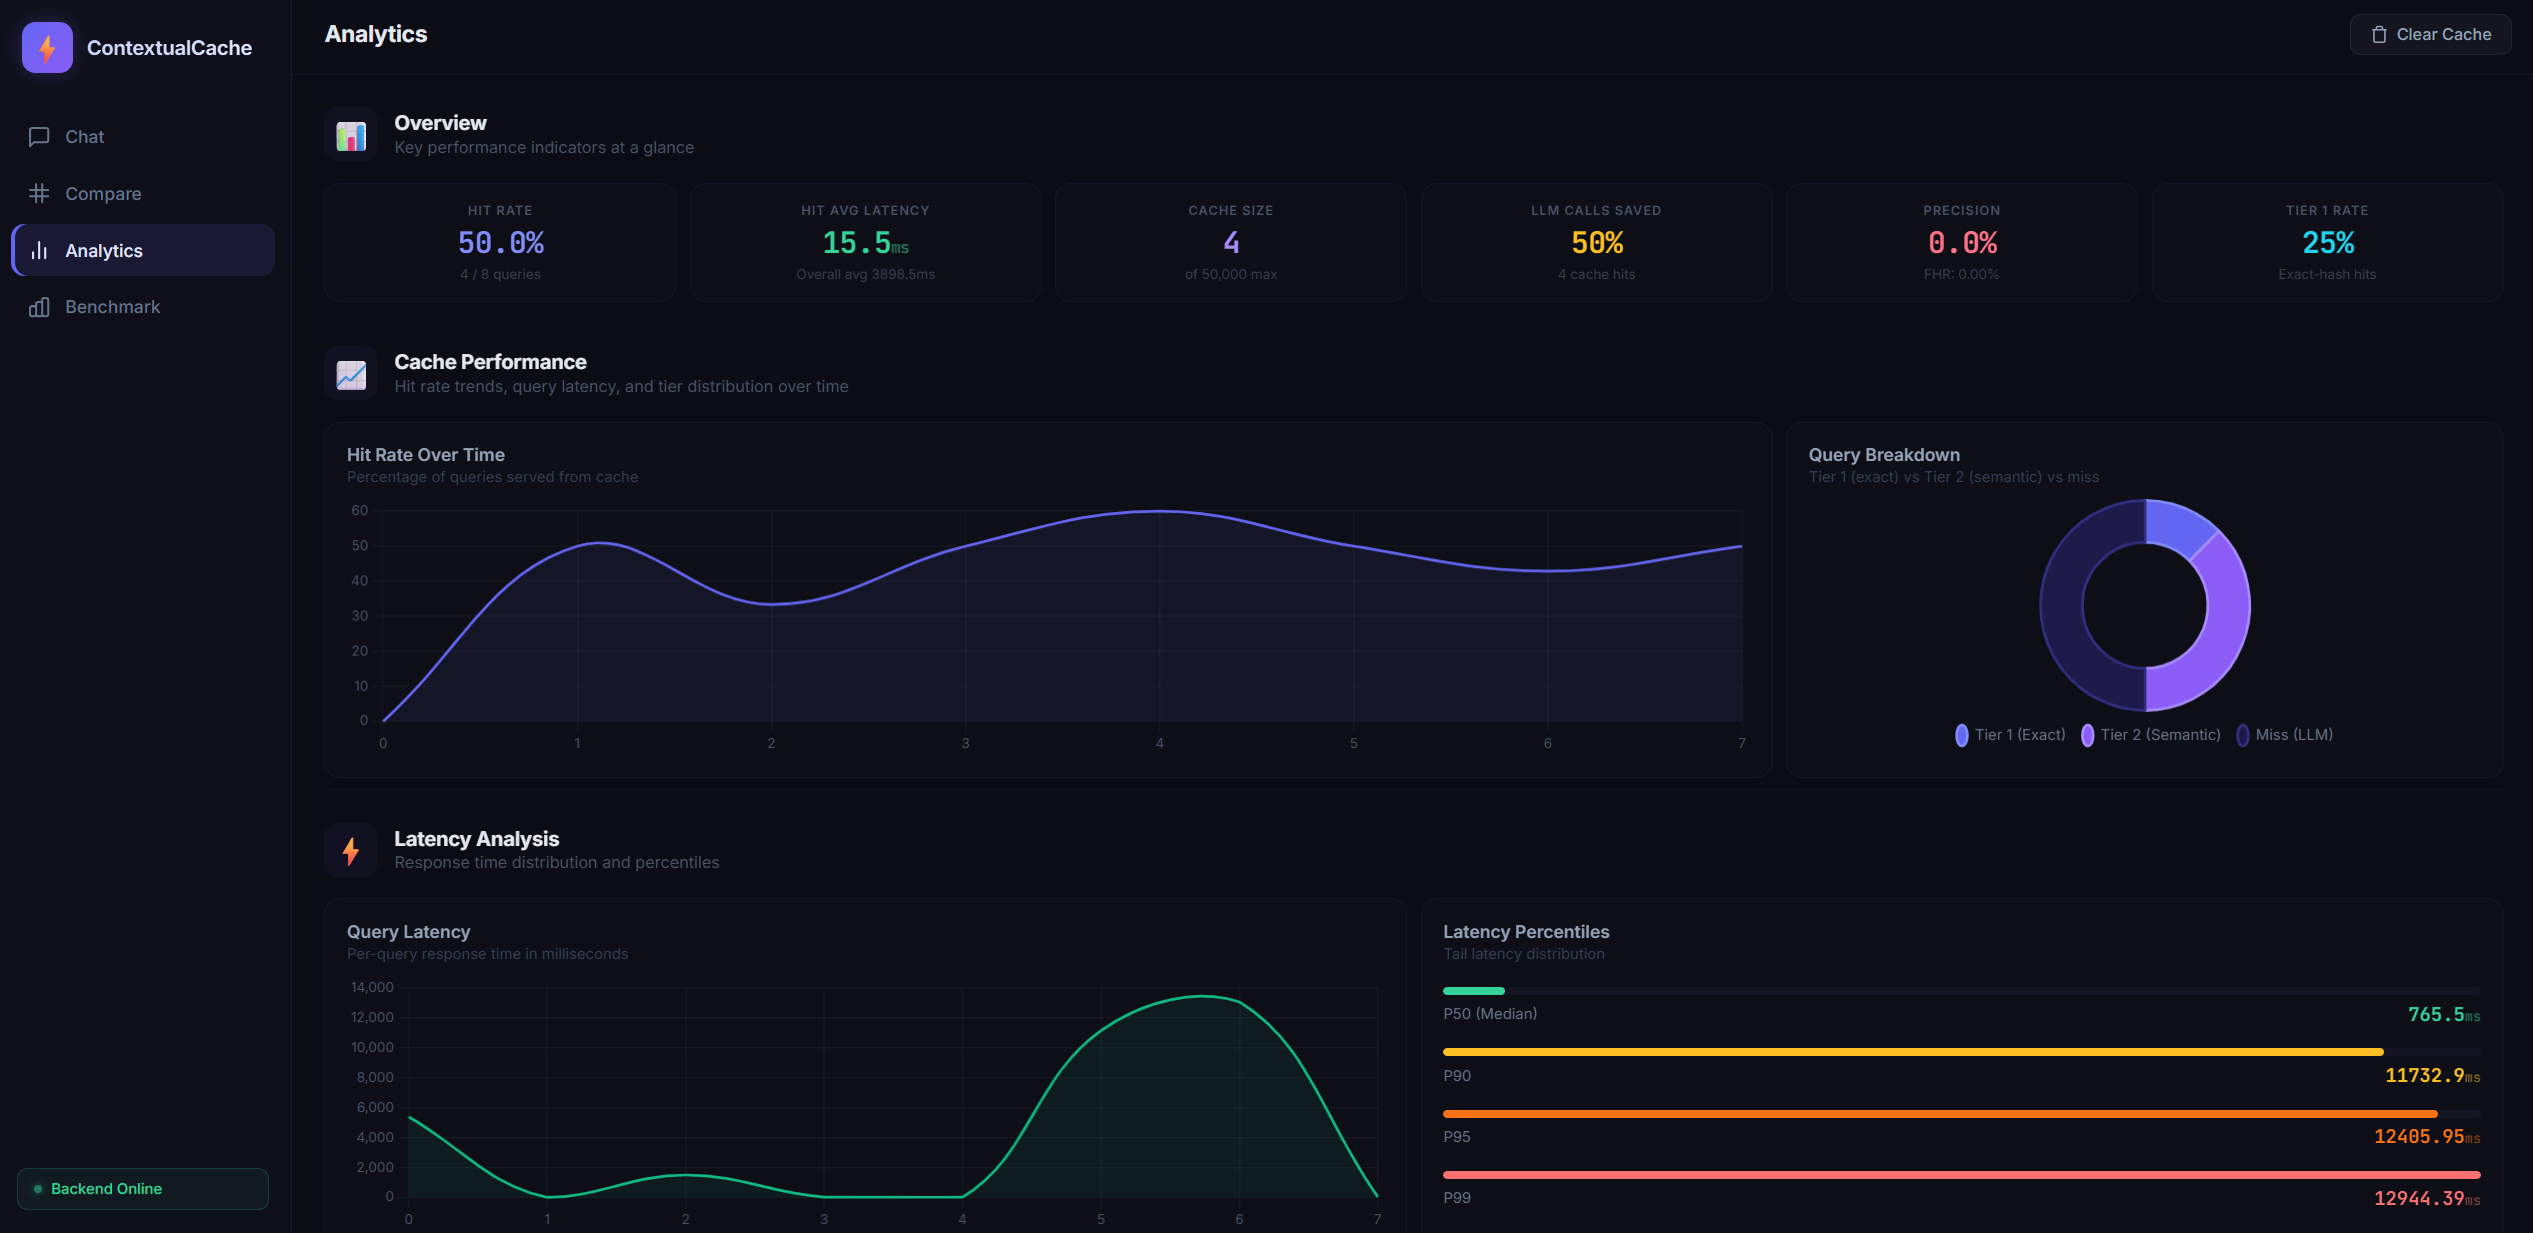
\includegraphics[width=1.0\textwidth]{fig-analytics-dashboard.png}
\caption*{Figure~\ref{fig:analytics}: Analytics dashboard with real-time monitoring}
\end{figure}

\begin{figure}[H]
\centering
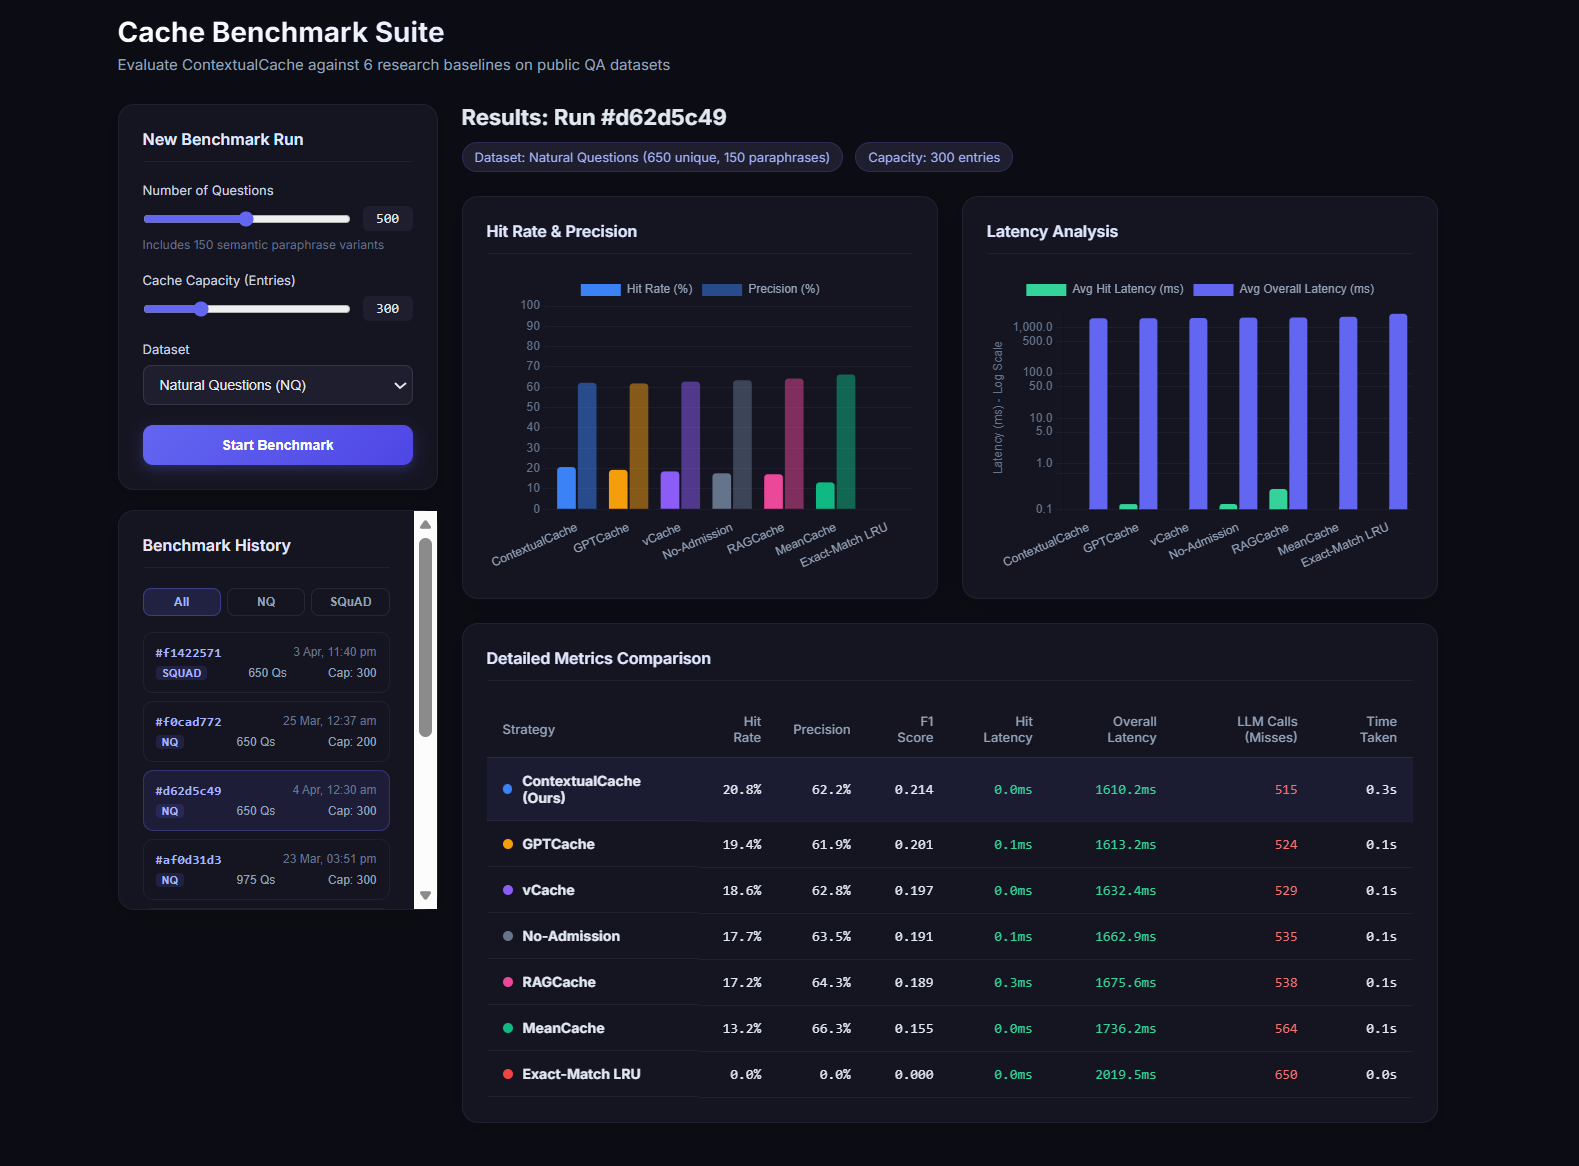
\includegraphics[width=0.9\textwidth]{fig-benchmark-suite.png}
\caption*{Figure~\ref{fig:benchmark}: Benchmark suite with dataset selection and results}
\end{figure}


% ════════════════════════════════════════════════════════════
% Appendix C: Tables
% ════════════════════════════════════════════════════════════
\newpage
\chapter*{Appendix C: Tables}
\addcontentsline{toc}{section}{Appendix C: Tables}

\vspace{0.3cm}
\noindent\textbf{Table~\ref{tab:litsurvey}: Literature Survey Summary}
\vspace{0.3cm}

\begin{longtable}{|c|p{2.5cm}|p{3cm}|p{3.5cm}|p{3.5cm}|}
\hline
\textbf{S.No.} & \textbf{Author} & \textbf{Approach} & \textbf{Key Contribution} & \textbf{Gap Identified} \\
\hline
\endfirsthead
\hline
\textbf{S.No.} & \textbf{Author} & \textbf{Approach} & \textbf{Key Contribution} & \textbf{Gap Identified} \\
\hline
\endhead
1 & Haqiq et al., 2025 & MinCache: Hybrid Cache & Three-tier hierarchy; 4.5$\times$ speedup vs GPTCache & MinHash misses nuanced semantics \\
\hline
2 & Gill et al., 2024 & MeanCache: User-Centric Caching & Federated learning for similarity models & No adaptive thresholds; fixed metrics \\
\hline
3 & Gao et al., 2025 & Online Context Caching & KV cache placement + request scheduling & Does not address semantic similarity \\
\hline
4 & Li et al., 2024 & SCALM: Semantic Caching & Vector quantization; semantic clustering & Semantic analysis overhead; no adaptation \\
\hline
5 & Li et al., 2024 & Context-based Semantic Caching & Context embedding + attention weighting & Increased memory footprint \\
\hline
6 & Liu et al., 2024 & Lost in the Middle & Position bias analysis in transformers & Affects compression, not caching \\
\hline
7 & Regmi \& Pun, 2024 & GPT Semantic Cache & Redis-based with HNSW ANN & Fixed threshold; lacks adaptability \\
\hline
8 & Jin et al., 2024 & RAGCache & Cost-aware GDSF eviction & No per-entry threshold adaptation \\
\hline
9 & Schroeder et al., 2025 & vCache & Per-entry conformal thresholds & High default; no bandit exploration \\
\hline
10 & Zha et al., 2023 & Online Optimization for Cache & Bayesian optimization for thresholds & Single query type; manual init \\
\hline
11 & Zhu et al., 2023 & Semantic Caching for LLM Cost & Embedding-based lookup & Fixed threshold $\tau$=0.8; no adaptation \\
\hline
12 & Einziger et al., 2017 & TinyLFU & Frequency-gated admission & Not designed for semantic caching \\
\hline
13 & Bifet \& Gavalda, 2007 & ADWIN & Adaptive windowing for drift & General-purpose; needs integration \\
\hline
14 & Vovk et al., 2005 & Conformal Prediction & Guaranteed prediction sets & Theoretical; per-entry adaptation needed \\
\hline
15 & McMahan et al., 2017 & FedAvg & Federated model averaging & Not applied to cache threshold learning \\
\hline
\end{longtable}

\vspace{0.5cm}
\noindent\textbf{Table~\ref{tab:pipeline}: Query Pipeline Complexity Analysis}
\vspace{0.3cm}

\begin{table}[H]
\centering
\begin{tabular}{llll}
\toprule
\textbf{Stage} & \textbf{Component} & \textbf{Complexity} & \textbf{Latency} \\
\midrule
Tier 1 & Exact Hash Lookup (SHA-256) & $O(1)$ & $<$1 ms \\
Tier 2 & FAISS HNSW Semantic Search & $O(\log n)$ & 2--15 ms \\
Embedding & paraphrase-MiniLM-L6-v2 & $O(d)$ & 5--20 ms \\
Threshold & Per-entry conformal $\tau_i$ & $O(k \log k)$ & $<$0.1 ms \\
Miss & LLM Provider (Ollama/Groq) & Network & 500--6000 ms \\
\bottomrule
\end{tabular}
\end{table}

\vspace{0.5cm}
\noindent\textbf{Table~\ref{tab:components}: Cache Management Component Summary}
\vspace{0.3cm}

\begin{table}[H]
\centering
\begin{tabular}{p{3cm}p{4.5cm}p{6cm}}
\toprule
\textbf{Component} & \textbf{Algorithm} & \textbf{Purpose} \\
\midrule
Admission & Semantic W-TinyLFU & Reject one-hit-wonders based on LSH-bucketed frequency \\
Eviction & CostGDSF & $H = f \times c / s + L$ (keeps expensive entries) \\
Threshold Learning & Thompson Sampling (10 arms) & Learn optimal default $\tau$ for new entries \\
Drift Detection & ADWIN & Reset bandit posteriors on distribution shift \\
Session Context & EMA fusion ($\alpha$=0.85) & Multi-turn conversational awareness \\
Fault Isolation & Circuit Breaker & Per-dependency isolation (CLOSED/OPEN/HALF\_OPEN) \\
\bottomrule
\end{tabular}
\end{table}

\vspace{2.4cm}
\noindent\textbf{Table~\ref{tab:arms}: Thompson Sampling Threshold Arms Configuration}
\vspace{0.3cm}

\begin{table}[H]
\centering
\begin{tabular}{cc}
\toprule
\textbf{Arm} & \textbf{Threshold Value} \\
\midrule
0 & 0.650 \\
1 & 0.683 \\
2 & 0.717 \\
3 & 0.750 \\
4 & 0.783 \\
5 & 0.817 \\
6 & 0.850 \\
7 & 0.883 \\
8 & 0.917 \\
9 & 0.950 \\
\bottomrule
\end{tabular}
\end{table}

\vspace{0.5cm}
\noindent\textbf{Table~\ref{tab:techstack}: Technology Stack}
\vspace{0.3cm}

\begin{table}[H]
\centering
\begin{tabular}{ll}
\toprule
\textbf{Category} & \textbf{Technology} \\
\midrule
Language & Python 3.10 \\
Backend Framework & FastAPI with Uvicorn ASGI \\
Embedding Model & paraphrase-MiniLM-L6-v2 (384d) \\
Vector Index & FAISS (faiss-cpu) with HNSW \\
LLM Backend & Ollama (LLaMA 3.2:3b) / Groq / OpenAI \\
Optional Cache Store & Redis (redis-py async) \\
Persistence & SQLite \\
Frontend Framework & SvelteKit (Svelte 5) \\
Desktop Runtime & Tauri (Rust) \\
Charting & Chart.js \\
Deep Learning & PyTorch (CUDA 12.6) \\
Testing & pytest with pytest-asyncio (120 tests) \\
\bottomrule
\end{tabular}
\end{table}

\vspace{4.5cm}
\noindent\textbf{Table~\ref{tab:api}: API Endpoint Summary}
\vspace{0.3cm}

\begin{table}[H]
\centering
\begin{tabular}{lll}
\toprule
\textbf{Method} & \textbf{Path} & \textbf{Description} \\
\midrule
POST & /query & Main cache-fronted LLM query \\
POST & /feedback & Correctness feedback for calibration \\
POST & /bulk-query & Batch queries \\
POST & /api/query-direct & Bypass cache, call LLM directly \\
GET & /health & Health check \\
GET & /api/stats & Full analytics for dashboard \\
POST & /api/clear-cache & Clear all cache entries \\
GET & /api/conversations & List chat sessions \\
POST & /api/benchmark/run & Start benchmark run \\
GET & /api/benchmark/status/\{id\} & Poll benchmark progress \\
GET & /api/benchmark/results & List benchmark results \\
\bottomrule
\end{tabular}
\end{table}

\vspace{0.5cm}
\noindent\textbf{Table~\ref{tab:config}: Configuration Parameters}
\vspace{0.3cm}

\begin{table}[H]
\centering
\begin{tabular}{lll}
\toprule
\textbf{Parameter} & \textbf{Value} & \textbf{Description} \\
\midrule
CC\_CACHE\_CAPACITY & 50,000 & Max cached entries (300 for benchmark) \\
CC\_DEFAULT\_THRESHOLD & 0.70 & Initial conformal threshold \\
CC\_TARGET\_ERROR\_RATE & 0.05 & Conformal error bound ($\varepsilon$) \\
CC\_EMBEDDING\_MODEL & MiniLM-L6-v2 & 384-dimensional embeddings \\
CC\_ANN\_K & 10 & FAISS top-$k$ neighbors \\
CC\_HNSW\_M & 32 & HNSW links per node \\
CC\_HNSW\_EF\_SEARCH & 64 & HNSW search expansion \\
CC\_WINDOW\_PCT & 0.05 & W-TinyLFU window fraction \\
CC\_CMS\_WIDTH & 4096 & Count-Min Sketch columns \\
CC\_BANDIT\_N\_ARMS & 10 & Thompson Sampling arms \\
CC\_DRIFT\_DELTA & 0.002 & ADWIN sensitivity \\
CC\_DEFAULT\_TTL\_S & 3600 & Entry time-to-live (seconds) \\
\bottomrule
\end{tabular}
\end{table}

\newpage

\noindent\textbf{Table~\ref{tab:nq}: Benchmark Results on Natural Questions Dataset (650 queries, 300 capacity)}
\vspace{0.3cm}

\begin{table}[H]
\centering
\begin{tabular}{lcccccc}
\toprule
\textbf{Strategy} & \textbf{Hit Rate} & \textbf{Precision} & \textbf{F1} & \textbf{Correct} & \textbf{Incorrect} & \textbf{LLM Calls} \\
\midrule
\textbf{Ours} & \textbf{20.77\%} & \textbf{62.22\%} & \textbf{0.214} & \textbf{84} & \textbf{51} & \textbf{515} \\
GPTCache & 19.38\% & 61.90\% & 0.201 & 78 & 48 & 524 \\
vCache & 18.62\% & 62.81\% & 0.197 & 76 & 45 & 529 \\
No-Admission & 17.69\% & 63.48\% & 0.191 & 73 & 42 & 535 \\
RAGCache & 17.23\% & 64.29\% & 0.189 & 72 & 40 & 538 \\
MeanCache & 13.23\% & 66.28\% & 0.155 & 57 & 29 & 564 \\
Exact-Match LRU & 0.00\% & --- & 0.000 & 0 & 0 & 650 \\
\bottomrule
\end{tabular}
\end{table}

\vspace{0.5cm}
\noindent\textbf{Table~\ref{tab:squad}: Benchmark Results on SQuAD Dataset (650 queries, 300 capacity)}
\vspace{0.3cm}

\begin{table}[H]
\centering
\begin{tabular}{lcccccc}
\toprule
\textbf{Strategy} & \textbf{Hit Rate} & \textbf{Precision} & \textbf{F1} & \textbf{Correct} & \textbf{Incorrect} & \textbf{LLM Calls} \\
\midrule
\textbf{Ours} & \textbf{23.69\%} & 35.71\% & \textbf{0.137} & \textbf{55} & 99 & \textbf{496} \\
GPTCache & 19.54\% & 38.58\% & 0.126 & 49 & 78 & 523 \\
vCache & 17.85\% & 38.79\% & 0.118 & 45 & 71 & 534 \\
No-Admission & 17.85\% & 37.07\% & 0.112 & 43 & 73 & 534 \\
RAGCache & 17.38\% & 36.28\% & 0.108 & 41 & 72 & 537 \\
MeanCache & 5.23\% & 47.06\% & 0.047 & 16 & 18 & 616 \\
Exact-Match LRU & 0.00\% & --- & 0.000 & 0 & 0 & 650 \\
\bottomrule
\end{tabular}
\end{table}

\vspace{0.5cm}
\noindent\textbf{Table~\ref{tab:precision}: Precision Analysis on NQ --- Top Three Strategies}
\vspace{0.3cm}

\begin{table}[H]
\centering
\begin{tabular}{lccc}
\toprule
\textbf{Metric} & \textbf{GPTCache} & \textbf{vCache} & \textbf{Ours} \\
\midrule
Total Hits & 126 & 121 & 135 \\
Correct Hits & 78 & 76 & 84 \\
Incorrect Hits & 48 & 45 & 51 \\
Precision & 61.90\% & 62.81\% & 62.22\% \\
False Positive Rate & 38.10\% & 37.19\% & 37.78\% \\
\bottomrule
\end{tabular}
\end{table}

\vspace{2.5cm}
\noindent\textbf{Table~\ref{tab:latency}: Latency Comparison on NQ}
\vspace{0.3cm}

\begin{table}[H]
\centering
\begin{tabular}{lccc}
\toprule
\textbf{Strategy} & \textbf{Hit Latency (ms)} & \textbf{Overall Latency (ms)} & \textbf{LLM Saved} \\
\midrule
Ours & 0.00 & 1610.17 & 135 \\
GPTCache & 0.13 & 1613.17 & 126 \\
vCache & 0.00 & 1632.40 & 121 \\
No-Admission & 0.13 & 1662.86 & 115 \\
RAGCache & 0.28 & 1675.60 & 112 \\
MeanCache & 0.00 & 1736.22 & 86 \\
\bottomrule
\end{tabular}
\end{table}


% ════════════════════════════════════════════════════════════
% Appendix D: Algorithms
% ════════════════════════════════════════════════════════════
\newpage
\chapter*{Appendix D: Algorithms}
\addcontentsline{toc}{section}{Appendix D: Algorithms}

\vspace{0.5cm}
\noindent\textbf{Algorithm 1: Conformal Threshold Update}
\vspace{0.3cm}

\begin{lstlisting}
Input: entry_id, similarity, was_correct
If was_correct:
    nonconformity = 1.0 - similarity
Else:
    nonconformity = min(1.0, max(1.0 - similarity + 0.1, 0.5))

scores[entry_id].append(nonconformity)
If len(scores) > max_window:
    scores = scores[-max_window:]

If len(scores) >= min_calibration_points:
    sorted_scores = sort(scores)
    idx = ceil((1 - epsilon) * (len + 1)) - 1
    tau_i = 1.0 - sorted_scores[idx]
    tau_i = clamp(tau_i, 0.60, 0.99)
Else:
    tau_i = default_threshold
\end{lstlisting}

\vspace{1cm}
\noindent\textbf{Algorithm 2: Thompson Sampling Update}
\vspace{0.3cm}

\begin{lstlisting}
On each cache hit:
    arm* = current best arm (highest expected reward)
    If similarity >= 0.85: reward = 1.0
    Else if similarity < 0.65: reward = 0.0
    Else: reward = (similarity - 0.65) / 0.20

    alpha[arm*] += reward
    beta[arm*] += (1.0 - reward)

    Feed reward to ADWIN drift detector
    If drift detected:
        Reset all alpha, beta to (2, 2)
\end{lstlisting}


\end{document}
